%% ----------------------------------------------------------------
%% Main.tex -- MAIN FILE (the one that you compile with LaTeX)
%% ---------------------------------------------------------------- 

% Set up the document
\documentclass[a4paper, 12pt, oneside]{Thesis}  % Use the "Thesis" style, based on the ECS Thesis style by Steve Gunn
\graphicspath{Figures/}  % Location of the graphics files (set up for graphics to be in PDF format)

% Include any extra LaTeX packages required
\usepackage[square, numbers, comma, sort&compress]{natbib}
\usepackage{verbatim}  % Needed for the "comment" environment to make LaTeX comments
\usepackage{vector}  % Allows "\bvec{}" and "\buvec{}" for "blackboard" style bold vectors in maths
\usepackage{amsmath}
\usepackage{physics}
\usepackage{hyperref}
\usepackage{bookmark}
\usepackage{amsmath,empheq}
\usepackage{caption}
\usepackage{pdfpages} 
\usepackage{tikz}
\usetikzlibrary{shapes, arrows, automata}
\usepackage{xcolor}
\usepackage{tabularx}
\usepackage{enumitem}
\usepackage[linesnumbered,ruled,vlined]{algorithm2e}
\usepackage[T1]{fontenc} %normes d'encodage
\usepackage[utf8]{inputenc} %normes d'encodage
\usepackage{lmodern} %correction d'affichage
\usepackage{graphicx} %insertion d'images
\usepackage{csquotes} %guillemets français
\usepackage{sectsty} %modifier l'apparence des titres
\usepackage{fancyhdr} %en tête et pieds de page personnalisables
\usepackage{etoolbox} %idem
\usepackage{color} %gestion des couleurs
\usepackage{setspace} %interligne
\usepackage{natbib} %pour pouvoir ne citer que l'année
\usepackage{chngcntr} %compteurs modifiables
\usepackage{amsmath} %package maths
\usepackage{amssymb} %package maths
\usepackage{url} %gestion des liens hypertextes
\usepackage{blindtext} %génération de texte aléatoire : \Blindtext
\usepackage{listings}
\lstset{
	frame=tb, % draw a frame at the top and bottom of the code block
	tabsize=4, % tab space width
	showstringspaces=false, % don't mark spaces in strings
	numbers=left, % display line numbers on the left
	commentstyle=\color{green}, % comment color
	keywordstyle=\color{blue}, % keyword color
	stringstyle=\color{red} % string color
}


%%% Coloring the comment as blue
\newcommand\mycommfont[1]{\footnotesize\ttfamily\textcolor{blue}{#1}}
\SetCommentSty{mycommfont}

\SetKwInput{KwInput}{Input}
\SetKwInput{KwOutput}{Output}

\hypersetup{urlcolor=blue, colorlinks=true}

%% ----------------------------------------------------------------
\begin{document}

% =======================================================================
%                              Title
% =======================================================================

%\title  {Towards Non-physical to Physical Interactions between Human-Humanoid Robot Co-workers }
%\setboolean{@twoside}{false}
% \includepdf[pages={1},width=\textwidth]{cover.pdf} 
% \includepdf[pages={1},offset=75 -75]{cover.pdf}

\thispagestyle{empty}


\begin{tikzpicture}[remember picture, overlay, shift=(current page.south)]
  \shade[top color=white , bottom color=gray] (current page.north west) rectangle (-3, 0);
\end{tikzpicture}

\begin{tikzpicture}[remember picture, overlay, shift=(current page.north west)]
    
    \node[inner sep=0pt] (thèse) at (15, -2)
    {\includegraphics[width=0.8\textwidth]{plots/cover/these.png}};
    
    \node[inner sep=0pt] (collegeDoctoral) at (5, -3)
    {\includegraphics[width=.225\textwidth]{plots/cover/doctoral.png}};
    
    \node[inner sep=0pt] (montpellier) at (5,-11)
    {\includegraphics[width=.225\textwidth]{plots/cover/montpellier.png}};
    
    \node[inner sep=0pt] (cnrs) at (5,-20)
    {\includegraphics[width=.225\textwidth]{plots/cover/cnrs.png}};
    
    \node[inner sep=0pt] (aist) at (5,-26)
    {\includegraphics[width=.25\textwidth]{plots/cover/aist.png}};
  

    \node[align=center] at (15,-10) {
    \\ \large 
    Délivrée par \textbf{
    l'Université de Montpellier %%%% UNIVERSITÉ %%%%
    }\\ \\ \\ \large 
    Préparée au sein de l'école doctorale I2S - Information,
    \\ \large 
    Structure, Systèmes % XX %%%% ÉCOLE DOCTORALE %%%%
    \\ \large 
    Et de l'unité de recherche UMR 5506 % XX %%%% UNITÉ DE RECHERCHE %%%%
    \\ \\ \\ \large 
    
    Spécialité : \textbf{
    SYAM - Systèmes Automatiques et
    }\\ \large 
    \textbf{
    Microélectroniques
    }\\ \\ \\ \\ \large 
    
    Présentée par : \textbf{
    Ashesh VASALYA
    }\\ \\};
    
    \node[draw, align=center] at (15, -17) {\, \hspace{12cm}
    \\ \Large \textbf{ 
    TITRE DE LA THÈSE} \\ \Large \textbf{ 
    SUR DEUX LIGNES   %%%% TITRE %%%%
    }\\ \large \textbf{
    sous-titre %%%% SOUS-TITRE %%%%
    }};
    
    \node[align=center] at (15, -20) {Soutenue le
    XX September 2019 %%%% DATE %%%%
    devant le jury composé de};
    
    \node[text width=12cm] at (15,-23) { %%%% JURY %%%%
    Civilité Prénom NOM, Grade, Etablissement \hfill Statut Jury \\
    Civilité Prénom NOM, Grade, Etablissement \hfill Statut Jury \\
    Civilité Prénom NOM, Grade, Etablissement \hfill Statut Jury \\
    Civilité Prénom NOM, Grade, Etablissement \hfill Statut Jury \\};
\end{tikzpicture}



%% ----------------------------------------------------------------

\frontmatter      % Begin Roman style (i, ii, iii, iv...) page numbering

\setstretch{1.3}  % It is better to have smaller font and larger line spacing than the other way round

% Define the page headers using the FancyHdr package and set up for one-sided printing
\fancyhead{}  % Clears all page headers and footers
\rhead{\thepage}  % Sets the right side header to show the page number
\lhead{}  % Clears the left side page header

\pagestyle{fancy}  % Finally, use the "fancy" page style to implement the FancyHdr headers

\clearpage
%% ----------------------------------------------------------------
% Declaration Page required for the Thesis, your institution may give you a different text to place here
\Declaration{

\addtocontents{toc}{\vspace{1em}}  % Add a gap in the Contents, for aesthetics

I, AUTHOR NAME, declare that this thesis titled, `THESIS TITLE' and the work presented in it are my own. I confirm that:

\begin{itemize} 
\item[\tiny{$\blacksquare$}] This work was done wholly or mainly while in candidature for a research degree at this University.
 
\item[\tiny{$\blacksquare$}] Where any part of this thesis has previously been submitted for a degree or any other qualification at this University or any other institution, this has been clearly stated.
 
\item[\tiny{$\blacksquare$}] Where I have consulted the published work of others, this is always clearly attributed.
 
\item[\tiny{$\blacksquare$}] Where I have quoted from the work of others, the source is always given. With the exception of such quotations, this thesis is entirely my own work.
 
\item[\tiny{$\blacksquare$}] I have acknowledged all main sources of help.
 
\item[\tiny{$\blacksquare$}] Where the thesis is based on work done by myself jointly with others, I have made clear exactly what was done by others and what I have contributed myself.
\\
\end{itemize}
 
 
Signed:\\
\rule[1em]{25em}{0.5pt}  % This prints a line for the signature
 
Date:\\
\rule[1em]{25em}{0.5pt}  % This prints a line to write the date
}
\clearpage  % Declaration ended, now start a new page

%% ----------------------------------------------------------------
% The "Funny Quote Page"
\pagestyle{empty}  % No headers or footers for the following pages

\null\vfill
% Now comes the "Funny Quote", written in italics
\textit{``Write a funny quote here.''}

\begin{flushright}
If the quote is taken from someone, their name goes here
\end{flushright}

\vfill\vfill\vfill\vfill\vfill\vfill\null
\clearpage  % Funny Quote page ended, start a new page
%% ----------------------------------------------------------------

% The Abstract Page
%\addtotoc{Abstract}  % Add the "Abstract" page entry to the Contents
%\abstract{
\addtocontents{toc}{\vspace{1em}}  % Add a gap in the Contents, for aesthetics
\section*{\huge Abstract}
%\ldots


\clearpage  % Abstract ended, start a new page
%% ----------------------------------------------------------------

\setstretch{1.3}  % Reset the line-spacing to 1.3 for body text (if it has changed)

% The Acknowledgements page, for thanking everyone
\acknowledgements{
\addtocontents{toc}{\vspace{1em}}  % Add a gap in the Contents, for aesthetics

The acknowledgements and the people to thank go here, don't forget to include your project advisor\ldots

}
\clearpage  % End of the Acknowledgements
%% ----------------------------------------------------------------

\pagestyle{fancy}  %The page style headers have been "empty" all this time, now use the "fancy" headers as defined before to bring them back

%% ----------------------------------------------------------------
\lhead{\emph{Contents}}  % Set the left side page header to "Contents"
\tableofcontents  % Write out the Table of Contents

%% ----------------------------------------------------------------
\lhead{\emph{List of Figures}}  % Set the left side page header to "List if Figures"
\listoffigures  % Write out the List of Figures

%% ----------------------------------------------------------------
\lhead{\emph{List of Tables}}  % Set the left side page header to "List of Tables"
\listoftables  % Write out the List of Tables

%% ----------------------------------------------------------------
\setstretch{1.5}  % Set the line spacing to 1.5, this makes the following tables easier to read
\clearpage  % Start a new page
\lhead{\emph{Abbreviations}}  % Set the left side page header to "Abbreviations"
\listofsymbols{ll}  % Include a list of Abbreviations (a table of two columns)
{
% \textbf{Acronym} & \textbf{W}hat (it) \textbf{S}tands \textbf{F}or \\
\textbf{LAH} & \textbf{L}ist \textbf{A}bbreviations \textbf{H}ere \\
}

%% ----------------------------------------------------------------
\clearpage  % Start a new page
\lhead{\emph{Physical Constants}}  % Set the left side page header to "Physical Constants"
\listofconstants{lrcl}  % Include a list of Physical Constants (a four column table)
{
% Constant Name & Symbol & = & Constant Value (with units) \\
Speed of Light & $c$ & $=$ & $2.997\ 924\ 58\times10^{8}\ \mbox{ms}^{-\mbox{s}}$ (exact)\\
}

%% ----------------------------------------------------------------
\clearpage  %Start a new page
\lhead{\emph{Vasalya A.}}  % Set the left side page header to "Symbols"
\listofnomenclature{lll}  % Include a list of Symbols (a three column table)
{
% symbol & name & unit \\
$a$ & distance & m \\
$P$ & power & W (Js$^{-1}$) \\
& & \\ % Gap to separate the Roman symbols from the Greek
$\omega$ & angular frequency & rads$^{-1}$ \\
}
%% ----------------------------------------------------------------
% End of the pre-able, contents and lists of things
% Begin the Dedication page

\setstretch{1.3}  % Return the line spacing back to 1.3

\pagestyle{empty}  % Page style needs to be empty for this page
\dedicatory{For/Dedicated to/To my\ldots}

\addtocontents{toc}{\vspace{2em}}  % Add a gap in the Contents, for aesthetics

%% ----------------------------------------------------------------
\mainmatter	  % Begin normal, numeric (1,2,3...) page numbering
\pagestyle{fancy}  % Return the page headers back to the "fancy" style

% Include the chapters of the thesis, as separate files
% Just uncomment the lines as you write the chapters

%\chapter{Introduction}

This thesis work is about the interactions between human and humanoid robot as co-workers in the industrial scenarios. By interactions, we started with a non-physical human-robot interaction based on a industrially inspired \textit{Pick-n-Place} task example and try to move towards physical human-robot interactions with an example of human humanoid dual arm bi-directional object handover.

\section{Reader's Guide}

\paragraph{chapter 1:}
talk little about each chapter

\paragraph{chapter 2:}

\paragraph{chapter 3:}


%2.1.6 Challenges for the application to pHRI: reasons for a haptic language
%thesis paul-evrard % Introduction
%\chapter{State-of-the-art}


%thesis agravante
%1.1.1Terminology with a cognitive and behavioral science

%perspective

\section{Behavioural Neuroscience}

\section{Cognitive Robotics}

\section{Motor Contagions}

\section{Humanoid Robots}
\subsection{Humanoid robot control}
\subsection{Locomotion and walking principles}
\subsection{Walking with physical interaction}


\section{Human Robot interaction: Physical \& Non-Physical}

 % S-O-T-A
%\input{plots/Chapter3} % PLosOne morethan
%\chapter{More than just co-workers}
%Motor Contagions Influence Performance

\section{Introduction}
Robotics is now increasingly shifting to service and application fields, where robots need to collaborate with, and work in close proximity to, human co-workers. In these scenarios, it is of prime importance to understand how the presence of a robot co-worker influences the performance of humans around them. This understanding is essential not just in regard to productivity, but also in order to monitor and control any emotional and motor effects the presence of robot co-workers may have on the humans.

Observation of actions performed by others is known to induce implicit effects on an individual's action. These effects, that are referred to as motor contagions, have been extensively studied in psychology and sports science~\cite{Heyes:PB:2011,Blakemore:Neuropsychologia:2005,Becchio:BJN:2007,Ganesh:Springer:2015,Ikegami:SciReport:2014,Hillebrandt:SciReports:2014,Chaminade:BRB:2008,Oztop:RAS_ICHR:2004,Kilner:CurBio:2003,Sciutti:IJSR:2012}. In comparison, studies of motor contagions during human-robot interactions~\cite{Vasalya:roman:2018} are sparse, and have examined either how the observation of robots affect a human's movement velocity~\cite{Noy:B&C:2009,Kilner:SocialNeuro:2007,Bisio:PlosOne:2010,Bisio:PlosOne:2014}, or how it affects a human's movement variance~\cite{Kupferberg:Methods:2009,Kupferberg:PlosOne:2012,Brass:ActaPsych:2001,Press:CBR:2005}. However, the studies that reported changes in movement variance utilize arguably abstract tasks, and the studies reporting changes in movement speed do not analyze at how the participant movement variance changed with the speed. On the other hand, most industrial tasks require specific precisions in the movements and therefore, the performance in these tasks needs to be defined by considering both task speed (or frequency) and task accuracy. Here primarily, we analyzed how looking at a robot affects both, the speed and variance of the observing human's movement, to see whether we can quantify how human \textit{performance} is affected by motor contagions.  
Furthermore, while there is contradictory evidence to suggest that the physical form of a robot co-worker (specifically whether it is humanoid or not) does~\cite{Chaminade:JPP:2009} or does not~\cite{Kupferberg:PlosOne:2012} affect the variance of movements by human's, it is unclear whether this is also true for the case of movements speeds, and hence performance. Finally, it is unclear whether and how the performance effects due to a robot co-worker are modulated by a human co-worker's prior experience with robots, an issue that is crucial to understand how the human performance will change with continued exposure to a robot co-worker.


To address these issues, we examined an empirical repetitive industrial task in which a human participant and a humanoid robot work near each other, see Fig.~\ref{fig:setup}. We systematically varied the behavior, specifically frequency of robot movements and examined whether and how the frequency of movements by the human participants, and their task accuracy, is affected by the presence of the robot. To investigate the effect of physical form, we added conditions where the robot co-worker torso and head were covered, and only the moving arm was visible to the human participants. Finally, in order to compare the humanoid co-worker to a human co-worker, we also checked how the effects on the participants changed with a human co-worker, with and without his/her torso and head visible. To anticipate our results, we found that the presence of a humanoid co-worker can affect human performance, but only when it's humanoid form is visible. Furthermore, the effect was observed to increase with prior robot experience by the humans.

%\begin{figure}[hpt]
%	\centering{\includegraphic/s[width=\columnwidth]{Chapters/c4-plots/setup}}
%	\caption{{\bf Experimental setup.} The participants in our experiment worked in six conditions; with a robot performing \textit{biological} movements in A) robot co-worker condition; B) human co-worker condition; to check relevance of  human form in C) robot covered co-worker condition; and D) human covered co-worker condition; E) a robot co-worker performing \textit{non-biological} movements in robot non-biol co-worker condition; F) a robot co-worker performing industrial movements. The coordinate axis defining the movement setup is indicated in white (A).}
%	\label{fig:setup}
%\end{figure}



\section{Materials and methods} \label{methods}

\subsection{Participants}

% For figure citations, please use "Fig" instead of "Figure".
A total of 45 healthy adults participated in our study. 3 participants (2 males and a female of 3 nationalities, 29.6$\pm$5, mean$\pm$SD, aged 25-35) worked as volunteer models for the capture of human arm motion data. 42 participants (20 Males and 22 females of 12 nationalities, 25.9$\pm$4.35, mean$\pm$SD, min. age 20, max. age 39), were participated as `co-workers' in our main experiment. 3 out of 45 participants were left-handed according to the {\it Edinburgh Handedness Inventory}, and all participants had normal or corrected to normal vision. The experiments were approved by the local ethics committee at the National Institute of Advanced Industrial Science and Technology (AIST) in Tsukuba, Japan, and all participants read and signed an informed consent form along with the PLOS consent form for the usage of their images in the paper before taking part in the experiments. Participants were well instructed and informed with the experiment and task procedure, however they were na\"ive to the motives (participants were not told what aspect of their behavior we were analyzing in the experiment) of the experiments to avoid bias in the results as we are interested in the implicit effect of motor contagion. Each Participant received 2021 Japanese Yen (JPY) to participate. 
Participants for our study were recruited through an advertisement via a local event forum, Facebook page of our experiment and via word of mouth in the Tsukuba University, Tsukuba, Japan. Participants needed to be at least 18 years old to participate in this experiment, apart from that, there were no restrictions.

\subsection{Setup}

The participant and co-worker (a human or a humanoid robot) were seated on a chair with tables facing each other as shown in the experiment setup (Fig.~\ref{fig:setup}). On a horizontally placed touch-screen (23-inch HD DELL, P2314T) on the table, participants were presented with two red circles of diameter $\oslash$5 cm at distance of 50 cm from each other. The co-worker was similarly presented with two red circles on black cardboard $\oslash$9 cm at distance of 50 cm. The whole setup was enclosed by movable panels and the panel behind the co-worker was covered with a dark grey curtain. A motion tracking system (Motion Analysis Co.) with six infrared cameras (kestrel) and ten passive markers were used to record the arm motions of the participant and co-worker at 200Hz. A bipedal HRP-2Kai~\cite{Kaneko:RAS_ICHR:2015} humanoid robot (154 cm tall, 58 kg, 32 degrees of freedom) was used as the robot co-worker (Fig.~\ref{fig:setup}). A well-trained experimenter (M, 37) acted as the human co-worker. Both co-workers used their right arm throughout the experiment.

\subsection{Experimental task and conditions}


Motivated by the hand movements during an industrial pick-and-place, or parts assembly task, our task required participants to repeatedly touch two static red circles on the touch-screen with a stylus in their right hand during the task (Fig.~\ref{fig:setup}). While the participants were asked to touch the circle in each trial, they were free to touch anywhere on the circle. In preliminary experiments, we found that the standard deviation of the participant's touches were less than 1 cm (both in the $x$ and $y$ directions), and we purposely chose the radius of the touched circles to be more than 2 times larger than their standard deviation (targets were of 5 cm in diameter). This large size was crucial because, while the participants were asked to touch the circle in each trial, they were free to touch anywhere on the circle. The large target size therefore enabled us to observe any change in participant's touch location (that may accompany contagions in their speed), in terms of position and standard deviation, across our experiment. 

A co-worker (human or HRP-2Kai) worked on the same task in front of the participants. The participants were asked to perform their task at their own chosen `comfortable' frequency, and ignore the co-worker. The participants worked in a series of 50 second trials with the co-worker. In a trial, participants initially performed alone for 10 seconds (participant-alone period), performed with the co-worker for next 20 seconds (together period) and then relaxed while watching the co-worker performs the task for the last 20 seconds (co-worker-alone period) (Fig.~\ref{fig:trialprotocol2}).   

\begin{figure}[hpt]
	\centering{\includegraphics[width=1\columnwidth]{Chapters/c4-plots/Fig2}}
	\caption{{\bf Trial protocol.} The participants worked in repeated trials with either a robot or human co-worker (the figure shows the trial with a robot co-worker). Each trial consisted of period when the participant worked alone and co-worker relaxed (participant-alone period), both worked together (together period), and the co-worker worked alone (co-worker-alone period). The notation of the time variable (represented in general by $\tau$) in each period are shown.}
	\label{fig:trialprotocol2}
\end{figure}

All participants wore ear buds and headphones (through which we sent white noise) and had no external audio feedback (confirmed in the post experiment questionnaire, Q6). They were instructed to ``{\it always hold the stylus like a stamp and touch alternatively inside each red circle on the touch-screen with continuous and smooth hand movements at a comfortable speed}''. They were specifically told to ``{\it focus on your own task and ignore the co-worker when he/it starts after them}''. No instructions were given regarding the speed and movement trajectory.

We studied six experimental conditions. The participants worked with a HRP-2Kai humanoid robot co-worker in four conditions, specifically, a) \textit{robot co-worker} in which the whole robot was visible to the participant, and the robot played back biological movements, b) \textit{robot covered co-worker}, in which the robot played back biological movements, but its head and torso were covered, such that the participant could only see the robot's moving arm. c) \textit{robot non-biol co-worker}, in which a fully visible robot performed \textit{non-biological} arm movements, d) \textit{robot indus co-worker}, in which a fully visible robot performed \textit{industrial} arm movements and they worked with a trained human experimenter in the remaining e) \textit{human co-worker} and f) \textit{human covered co-worker} (where the head and torso of the human experimenter were covered) conditions, (see subsection~\nameref{HRP2_Traj}).

The experiment for each participant consisted of working in 3 conditions. Each participant was assigned to one of 6 \emph{condition combination} groups, see Table~\ref{groupTable}, each with the robot co-worker condition (main), in addition to two out of five other conditions. The order of the conditions was balanced across the combination groups. This allowed us to compare the behavior of the same participants in each condition in a combination group, with their behavior in the robot co-worker condition.


\begin{table}[hpt]
	\caption{condition combination groups (G)}
	{HRP-2Kai in robot co-worker (RV), robot covered co-worker (RC), robot non-biol co-worker (RN), robot indus co-worker (RI) conditions and Human experimenter in human co-worker (HV), human covered co-worker (HC) conditions. The order of conditions in a combination group were randomized across participants.}
	\label{groupTable}
	\begin{center}
		\begin{tabular}{|c cccccc|}
			\hline  
			{\bf Sessions/Groups} &  {\bf G1} &  {\bf G2} &  {\bf G3} &  {\bf G4} &  {\bf G5} &  {\bf G6}  \\ 
			\hline
			Session 1 & RI & RC & HV & RC & RN &  RC \\ 
			
			Session 2 & RV & RI & RV & HC & HV &  RN \\ 
			
			Session 3 & RN & RV & HC & RV & RV &  RV \\ 
			\hline 			
		\end{tabular} 
	\end{center}
\end{table}


Each condition had 10 trials. The co-worker performed at a constant, pseudo-randomly selected frequency (in the range of 0.16 to 1.1 Hz) in each trial. The pseudo-random nature of the co-worker performance was critical to avoid behavioral drift contamination across trials. The human co-worker was provided with a metronome using earphones like in~\cite{Bisio:PlosOne:2014}, to cue and help maintaining the movement frequency in each trial.

The robot movements in the robot co-worker conditions were a playback of the movements recorded from a previous human volunteer (see subsection~\nameref{HRP2_Traj} for details). We quantified the participant performance in the trials by their half time periods or {\it htp} (the average time between two consecutive alternate touches, measured using motion tracking), and the variance of their press location (measured as a change of mean and standard deviation of their touch-screen presses in the X-Y plane).

\subsection{HRP-2Kai movement trajectories} \label{HRP2_Traj}


The biological movements played on HRP-2Kai in robot co-worker and robot covered co-worker conditions were a playback of the human arm movements (Fig.~\ref{fig:trajectories}, blue plot) recorded in a preliminary experiment with three volunteers using the same (Motion Analysis Co.) motion tracking system, while the human movements were cued by an audio metronome. Movements were collected at several frequencies between 0.16 to 1.1Hz. We found the movements of the three volunteers to be statistically similar in the Cartesian velocity profiles (p$>$0.05), and showing similar trend in movement height with movement frequency --trajectory height consistently decreased with increase of movement frequency. We therefore chose to use the movements recorded from one volunteer (a male) in this experiment.


\begin{figure}[hpt]
		\centering{\includegraphics[width=\columnwidth]{Chapters/c4-plots/Fig3}}
	\caption{{\bf HRP-2Kai movement trajectories.} The trajectories played by the robot in robot co-worker, robot covered co-worker, robot non-biol co-worker and robot indus co-worker conditions.}
	\label{fig:trajectories}
\end{figure}


Well learnt human movements are characterized by a bell-shaped velocity profile. The peak of the bell-shaped profile may be shifted forward in time when precision is required at the reach end (like in our task when the participants required to touch inside a given target region), but the velocity profile is normally characterized by a single peak. Therefore, to develop a `non-biological' movement profile for the robot non-biol co-worker condition, we developed a movement profile with multiple velocity peaks. This profile was developed in position-time (cyan plots in Figs.~\ref{fig:trajectories} and~\ref{fig:trajectories2}) profile using fifth and third order polynomial segments (lift-off, carry, set-down)~\cite{Biagiotti:Springer:2008}. We observed that human volunteers' movements to predominantly be in the Y-Z plane. The piece-wise polynomial trajectory for the robot non-biol co-worker condition was designed over the $y$ (horizontal) and $z$ (vertical) dimensions, while $x$ was always kept constant zero.


\begin{figure}[hpt]
		\centering{\includegraphics[width=\columnwidth]{Chapters/c4-plots/Fig4}}
	\caption{{\bf HRP-2Kai trajectory generation.} The time trajectories in the Y and Z axis by the HRP-2Kai in the robot non-biol co-worker and robot indus co-worker condition, and the via-points (blue circles) used to generate both trajectories.}
	\label{fig:trajectories2}
\end{figure}


The industrial trajectory was characterized by a constant velocity phase. Inspired from the industrial manipulators, and keeping in mind our HRP-2Kai joint constraints during fast movements, we improvised the traditionally used industrial trapezoidal velocity profile, with a third order velocity sections in the acceleration and deceleration phase (magenta plots in Figs.~\ref{fig:trajectories} and~\ref{fig:trajectories2}). Again, since our movements were restricted in the Y-Z plane, we designed our smooth trapezoidal trajectory over the $y$ (horizontal) and $z$ (vertical) dimensions, while $x$ is kept constant and zero. The Z elevation ($z_{\max}$) in this trajectory was set to 13~cm when the robot moved from left to right, and 8 cm during the return.


\subsection{Variables}

Our analysis is based on the position data from both the participant's and co-worker's stylus markers. To extract out possible behavioral differences between the movements forward and backward, between the touch points, we analyzed behavioral variables across each movement between the red circles on the touch-screen, which we call as iterations (such that two iterations make a movement cycle). As participants and co-workers were required to make non-stop continuous movements between touches, we could extract individual iterations of participant's and co-worker's by looking for changes in the direction of $y$-velocity in the recorded motion capture data. In this study, we were interested in the task performance of participants, and therefore we primarily concentrated on the time between the alternate touches in each iteration, which we refer to as the half-time period ({\it htp}) or $\tau$, and the location of their touches on the touch-screen (in the X-Y plane). In addition, we also analyzed various measures of position, velocity and acceleration along the Y (horizontal) and Z (vertical) axes over each iteration. However, these results are out of scope of this study.

\subsection{Data analysis} \label{data_analysis}

We quantified the motor contagion in a participant' {\it htp} (the average time between two consecutive alternate touches) by analyzing the change of participant's {\it htp} between the together period and alone-period (see Fig.~\ref{fig:trialprotocol2}) in a trial ($\tau_p^t(i)-\tau_p^a(i)$), relative to the {\it htp} of the co-worker behavior in the same trial ($\tau_c (i)-Av(\tau_p^a)$), where $Av(\tau_p^a)$ represents the average undisturbed {\it htp} by a participants across his/her participant-alone periods. This data was regressed with either a first or second order regression model that was chosen based on the Akaike Information Criteria (AIC)~\cite{Akaike:ISIT:1973} and by using MATLAB's {\tt fitlm} function for each participant. The tangent slope at the minimum data abscissa value ($\min[\tau_c(i)-Av(\tau_p^a)]$) was collected across participants, checked for normality using the Shapiro-Wilk test and then analyzed for difference from zero using a one sample T-test (in case the distribution was normal) or a Signed Rank test. The fitting of {\it htp} in one sample participant from each of the six reported conditions are shown in Fig.~\ref{fig:allfit}, and the plot of the collection of slopes are in shown in Fig.~\ref{fig:slope_allcond}. A similar procedure was used to analyze the change in a participant's average X press location, average Y press location, standard deviation of X press location, and standard deviation of Y press locations relative to the {\it htp} of the co-worker behavior in the same trial ($\tau_c(i)-Av(\tau_p^a)$). The slopes from these analysis are shown in Fig.~\ref{fig:variance}.

\begin{figure}[hpt]
		\centering{\includegraphics[width=1\columnwidth]{Chapters/c4-plots/Fig5}}
	\caption{{\bf Examples of linear regression  fits.} The change of participant's {\it htp} (the average time between two consecutive alternate touches) between the together period and alone-period ($\tau_p^t(i)-\tau_p^a(i)$), relative to the {\it htp} of the co-worker behavior in the same trial ($\tau_c (i)-Av(\tau_p^a)$), where $Av(\tau_p^a)$ represents the average undisturbed {\it htp} by a participant across all his/her participant-alone periods. Note that the (robot or human) co-worker {\it htp} was random across trials, and the data in plots here are the ensemble of the participant behaviors arranged in increasing co-worker's {\it htp} on the abscissa. Each plot represent a condition, A) robot co-worker (blue); B) human co-worker (orange); C) robot covered co-worker (dark blue); D) human covered co-worker (dark orange); E) robot non-biol co-worker (cyan); F) robot indus co-worker (magenta) conditions. We used the AIC to choose either a first or second order model to fit the data for each participant. The lines represent the tangent slopes at the minimal data abscissa value.}
	\label{fig:allfit}
\end{figure}


\begin{figure}[hpt]
		\centering{\includegraphics[width=1\columnwidth]{Chapters/c4-plots/Fig6}}
	\caption{{\bf All six conditions \textit{htp} comparision.} The plot of the collection of slopes which is obtained in Fig.~\ref{fig:allfit} and ~\nameref{S1_Fig} to~\nameref{S6_Fig} supplementary figures. The condition-wise comparison of the change of participants {\it htp} with co-worker {\it htp}. P-values are Bonferroni corrected where required. The tangent slope at the minimum data abscissa value ($\min[\tau_c(i)-Av(\tau_p^a)]$) was collected across participants (as shown in Fig.~\ref{fig:allfit}), checked for normality using the Shapiro-Wilk test and then analyzed for difference from zero using a one sample T-test (in case the distribution was normal) or a Signed Rank test.}
	\label{fig:slope_allcond}
\end{figure}



\begin{figure}[hpt]
		\centering{\includegraphics[width=1\columnwidth]{Chapters/c4-plots/Fig7}}
	\caption{{\bf Participants touch variance.} Change of participant touch position with A) robot co-worker {\it htp}; B) human co-worker {\it htp}. A similar procedure which was used to quantify {\it htp} was also used here (see subsection~\nameref{data_analysis}) to analyze the change in a participant's average X press location, average Y press location, standard deviation of X press location, and standard deviation of Y press locations relative to the {\it htp} of the co-worker behavior in the same trial.}
	\label{fig:variance}
\end{figure}


Next, to check the relevance of the human form, we conducted the robot covered co-worker and human covered co-worker conditions, in which the head and torso of the co-worker was covered and only the moving arm was visible to the human (see Fig.~\ref{fig:setup}C, D or inset photos in Fig.~\ref{fig:slope_allcond}). All other experimental settings and analysis were same as in the robot co-worker and human co-worker conditions.


\subsection{Participant sample size}

As the effects of the robot co-worker condition was the focus of our experiments, each of our participant worked in the robot co-worker condition, and two of the remaining 5 conditions (human co-worker, robot covered co-worker, human covered co-worker, robot non-biol co-worker and robot indus co-worker). Note that due to the fact that each of our conditions lasted over 20 minutes, resulting in more than 1 hour of total experiment time for the three conditions, we could not have every participant participating in all the conditions. We initially recruited 35 participants to have 14 participants in each of the five conditions (giving five participant groups each of whom participated in one of the five conditions in addition to the robot co-worker condition), so as to enable a intra participant one sample T-test between the robot co-worker and each of the remaining conditions. The number `14' was chosen as it corresponds to participant numbers in similar previous studies~\cite{Bisio:PlosOne:2010,Bisio:PlosOne:2014} and corresponds to a power analysis using G* power for a 2-tailed, one sample T-test ($\alpha$=0.05, $\beta$=0.85, $d$=0.9)~\cite{Erdfelder:JBRMIC:1996, Verma:power_analysis:2017}. However, we found that with these participant numbers, the slopes in the same robot co-worker condition were not similar among the participant groups (p\textless 0.05, one-way ANOVA). The robot co-worker condition slopes were significantly different from zero with two participant groups (p=0.022, and p=0.038), tended to be significant in two (p=0.07, and p=0.08) and not significant in another (p=0.36). As a majority of the values tended to be significant, we decided to increase the participant numbers by 50\% (7 participants) across the participant group that were tending or not significant (these included participants who participated also in the robot covered co-worker, robot non-biol co-worker, and robot indus co-worker conditions), making a total of 42 participants. With this participant number, the robot co-worker {\it htp} slopes were observed to be similar across the participant groups (H(4), P=0.99; one-way Kruskal-Wallis H-test). After removal of three outliers, this gave us participants numbers of 13 (human co-worker condition), 13 (human covered co-worker), 17 (robot covered co-worker), 17 (robot non-biol co-worker), 18 (robot indus co-worker), and 39 in total for the robot co-worker condition, see Table~\ref{sizeTable}.

\begin{table}[hpt]
	\caption{Participant sample size}
	\label{sizeTable}
	\begin{center}
		\begin{tabular}{|c c|}
			\hline  
			{\bf condition} &  {\bf sample size} \\ 
			\hline
			robot co-worker & 39 \\ 
			\hline
			human co-worker & 13 \\
			\hline
			robot covered co-worker & 17 \\
			\hline
			human covered co-worker & 13 \\
			\hline
			robot non-biol co-worker & 17 \\
			\hline
			robot indus co-worker & 18 \\
			\hline 			
		\end{tabular} 
	\end{center}
\end{table}


\subsection{Questionnaire}

\subsubsection{Perception and fatigue}

Each of the participant in our experiment answered a short post experiment questionnaire consisting of 6 questions. The participants were asked to choose a score on a scale of 0 to 7, where 0 (Not at all), 7 (very strongly), for each of these questions, individually for every session they participated in:

\begin{enumerate}[start=1,label={Q\arabic*.}]
	\item My movements were affected when the agent was working with me.
	\item My movement speed was changed when the agent was working with me.
	\item I was tired during the experiment.
	\item I could maintain the movement speed that I wanted even when the robot was performing its task.
	\item I found it difficult to do my task when the agent was working with me.
	\item I could hear noises from the co-worker during the experiment.
\end{enumerate}

Q1, Q2, Q4 and Q5 were designed to access whether the participants cognitively realized the affects on their behavior due to the co-worker. A score close to one in Q1, Q2 and Q5 (and a score close to 7 in Q4) indicates that they did not consciously realize the effects. Therefore we considered the Q4 scores by subtracting the reported values from 7.

\subsubsection{Robot exposure questionnaire}

Following the end of our data collection, we also noted the need to measure the participant's robot experienced and exposure to robots. We therefore sent them a questionnaire of four questions:

\begin{enumerate}[start=1,label={RQ\arabic*.}]
	\item How many hours do you see and/or read about robots on average per week (include robots on TV)?
	\item If you work with robots currently, how many hours do you work with robots (or on robotics related topics) per week?
	\item If you have worked with robots, but do not work anymore, how many hours have you worked on them?
	\item How will you rate your knowledge of robots?
\end{enumerate}

For each question, the participant had to answer in hours and chose between `0', `less than 5', `5-10' `10-15', `15-20', `20-25', `25-30', `more than 30'.


\subsection{Statistical correction}

As reported earlier, every participant in our study participated in three conditions: the robot co-worker condition, and two of the remaining conditions. We thus compare the behavior of the participant in any condition with the robot co-worker. For each participant, there were thus two comparisons made. Correspondingly, in our comparisons in Fig.~\ref{fig:slope_allcond}, we use a Bonferroni correction of (3 conditions - 1) 2, and all p values below 0.05 were multiplied by 2. Therefore, note that all the comparisons between conditions in Fig.~\ref{fig:slope_allcond} are between equal number of participants (and we use a one sample T-test).

%%%%%%%%%%%%%%%%%%%%%%%%%%%%%%%%%%%%%%%%%%%%%%%%%%%%%%%%%%%%%%%%%%%%%%%%%%%%%%%%

% Results and Discussion can be combined.
\section{Results}


\subsection{Robot behavior influences human movement frequency}
Fig.~\ref{fig:allfit} shows the change of participant's {\it htp} (the average time between two consecutive alternate touches) between the together period and alone-period ($\tau_p^t(i)-\tau_p^a(i)$), relative to the {\it htp} of the co-worker behavior in the same trial ($\tau_c (i)-Av(\tau_p^a)$), where $Av(\tau_p^a)$ represents the average undisturbed {\it htp} by a participants across all his/her participant-alone periods. Note that the (robot or human) co-worker {\it htp} was random across trials, and the data in Fig.~\ref{fig:allfit} is an ensemble of the participant behaviors arranged in increasing co-worker's {\it htp} on the abscissa. We then collected the slope of the polynomial at the lowest data abscissa as a measure of how the participant {\it htp} was affected by the co-worker {\it htp}. In the robot co-worker condition the slope distribution was not normal across the participants (p$<$0.05, Shapiro-Wilk test, median=0.017) and was significantly positive across participants (median=0.017, Z(38)=3.70, p=0.0002, Signed Rank test). The positive slopes (light blue data in Fig.~\ref{fig:slope_allcond}) show that the robot performance {\it htp} (hence frequency) influenced the human participants. First, the human participant's {\it htp} increased when the robot {\it htp} was longer (see first quadrants of Fig.~\ref{fig:allfit}A), but for several participants, this increase had a threshold after which the participant's {\it htp} decreased. This behavior is the reason why we found a second order fit to explain the data better with many participants using AIC. Second, the participants {\it htp} also decreased when the robot {\it htp} was shorter (3rd quadrants of Fig.~\ref{fig:allfit}A, only across the participants in robot co-worker condition) indicating that a faster robot made the participants frequency higher. The {\it htp} results were similar with the human co-worker. The positive slopes (orange data in Fig.~\ref{fig:slope_allcond}) show that the human co-worker's performance {\it htp} (hence frequency) influenced the human participants (median=0.012, p=0.0017, Signed Rank test).





\subsection{Press accuracy in the human not affected by robot co-worker}

Studies in motor control have exhibited that human movements are constrained by motor noise, which increases with the magnitude of motor commands in the muscles~\cite{Harris:Nature:1998}. In the case of `regular' and automatic movements in daily life, this leads to a trade-off between the speed and accuracy of the movement~\cite{Fitts:JEP:1954}. However, the accuracy of movements is also modulated by the regulation of arm impedance by muscle co-contraction~\cite{Burdet:nature:2001, Franklin:JoN:2008, Ganesh:RAS:2013}. As mentioned earlier, to comment on the task performance of the human co-worker, we next analyzed whether and how the touch accuracy of the participants changed alongside the contagions in their {\it htp}. 

Again, note that the target circles provided to the participants were large (5~cm diameter), and there were no constraint on where inside the target they touched. Therefore the participant's touches can change (in position and/or variance) with their movement speed, without violating the task. However, interestingly we found that while the participants {\it htp} (hence movement frequency) changed, there were no such trend in the participants press (task) accuracy. 

The mean touch positions were ($\overline{X}$=0.95~cm; $\overline{Y}$=1.17~cm) from the circle center across the participants, and showed a mean standard deviations of (std(X)=0.23~cm; std(Y)=0.79~cm) (across participants) when they worked alone (in the participant-alone period). And crucially, the participants maintained the same touch positions (there was no change of mean touch positions $\overline{X}$: p=0.64; $\overline{Y}$: p=0.86) and mean standard deviations (change of std(X): p=0.56; std(Y): p=0.41) between when they worked alone and when they worked with the robot co-worker (Fig.~\ref{fig:variance}A), showing that the robot did not affect their task accuracies.

The press accuracy was similarly constant in the human co-worker condition in which the participants worked with another (unfamiliar) human, with no observed changes in the mean touch positions ($\overline{X}$: p=0.69; $\overline{Y}$: p=0.83; Fig.~\ref{fig:variance}B) and mean standard deviations (std(X): p=0.56; std(Y): p=0.39; Fig.~\ref{fig:variance}B). Here note again, that the touched circles were relatively large (5~cm) and the participants could have changed their touch position and variance while still satisfying the required task, but we do not observe this trend. Together, the change in movement frequency, and the lack of change in task accuracy shows that robot as well as human co-workers influenced participant task performance in our experiment.


\subsection{Human form matters}

Interestingly, covering the head and torso extinguished the contagions in the participant's {\it htp} --the participant's {\it htp}s were no longer affected in the robot covered co-worker (T(16)=-0.3, p=0.78; dark blue data in Fig.~\ref{fig:slope_allcond}) and the human covered co-worker (T(12)=0.24, p=0.82; dark orange data in Fig.~\ref{fig:slope_allcond}), and these effects were significantly lower than the effects induced in the same participants in the robot co-worker condition (T(16)=2.74, p=0.028, Bonferroni corrected, one sample T-test between robot co-worker and robot covered co-worker; T(12)=2.50, p=0.054, Bonferroni corrected, one sample T-test between robot co-worker and human covered co-worker). This result show that the human form is crucial for induction of the performance changes.

In the robot co-worker and robot covered co-worker conditions, the robot played back the biological arm movements of a previous human volunteers. Finally, corresponding to previous studies that have shown that motor contagions are attenuated when a robot makes non-biological movements~\cite{Kilner:CurBio:2003,Bisio:PlosOne:2014}, we added two control conditions (robot non-biol and robot indus) in which the participants could see the robot co-worker's whole upper body, but the robot made non-biologically inspired arms movements to perform the task (see subsection~\nameref{HRP2_Traj}). Consistent with previous studies we did not find any significant change in {\it htp}s in this condition (Z(16)=-1.07, p=0.29 (cyan data); Z(17)=-0.28, p=0.77 (magenta data) in Fig.~\ref{fig:slope_allcond}), and these values were different (tending to significance) compared to the robot co-worker condition of the same participants (robot non-biol condition: T(16)=2.32, p=0.066, Bonferroni corrected, one sample T-test) and (robot indus condition: T(17)=2.53, p=0.043, Bonferroni corrected, one sample T-test).


\subsection{The performance effect were implicit} \label{questionnaire}

An average of the scores from Q1, Q2, Q5 and Q4 (value subtracted from 7) was found to be equal to (mean$\pm$SD, 1.90$\pm$0.18) for the robot co-worker condition, and (mean$\pm$SD, 1.65$\pm$0.24) for the human co-worker condition respectively. These low scores suggested that the participants did not consciously realize the effects on their behavior. Q3 was used to confirm that the participants were not tired in our task. We obtained scores of (mean$\pm$SD, 0.96$\pm$0.18) across the participants in the robot co-worker condition, and (mean$\pm$SD, 0.75$\pm$0.22) in the human co-worker condition. Q6 was used to confirm that the participants did not hear any external audio cues from either the robot's joints in the robot co-worker conditions (mean$\pm$SD, 0.5$\pm$1.25), nor the human co-worker's touches in the human co-worker conditions (mean$\pm$SD, 0.58$\pm$1.36).

\subsubsection{Contagion increases with robot exposure}

We received answers from 23 participants on our robot exposure questionnaire. Out of these participants, one participant who scored `0' for all questions was removed. We averaged the scores (taking either one from RQ2 and RQ3, as they were complementary) for the others and plotted the average against their {\it htp} slope in the robot co-worker condition in Fig.~\ref{fig:corelation}. Interestingly, we observed a significant positive correlation (Pearson's R=0.44, p=0.039), such that the effect on the participants were larger if they had more exposure and experience with robots. This result is conform to a recent report where participants with more experience with robots show higher adaptation to it, see~\cite{vannucci:roman:2017}.


\begin{figure}[hpt]
		\centering{\includegraphics[width=1\columnwidth]{Chapters/c4-plots/Fig8}}
	\caption{{\bf Robot experience exposure.} The plot of the change of participant {\it htp}, with respect to their prior robot exposure and experience (self-scored by participants) showed a significant correlation between the two.}
	\label{fig:corelation}
\end{figure}


%%%%%%%%%%%%%%%%%%%%%%%%%%%%%%%%%%%%%%%%%%%%%%%%%%%%%%%%%%%%%%%%%%%%%%%%%%%%%%%%

\section{Discussion}
In summary, primarily, we observed that the performance frequencies of human participants were influenced by the presence of a humanoid robot co-worker (or a human co-worker). We observed that participants not only become slower with a slower co-worker, but also faster with faster co-workers. Here we were interested to see the change of participant behavior `relative' to the robot behavior. Hence we looked at a ratio, hence to quantify the motor contagion, we analyzed change in participant's \textit{htp} between the together period and alone-period in a trial and relative to the {\it htp} of the co-worker behavior in the same trial. When the numerator term ($\tau_p^t(i)-\tau_p^a(i)$) is negative that means participants get faster from their initial participant-alone period \textit{htp} (movement speed) and vice versa. Note that the subtraction in the denominator (of $Av(\tau_p^a)$ ) is a constant that only shifts the curve and does not effect the slope.  

In this study we wanted to choose a task that is simple, yet rich, and is representative of many industrial co-worker scenarios. We found that (repetitive) pick and place tasks to be the most common industrial tasks in which robots are employed. We therefore chose to start with a cyclic touch task in this experiment. The results we obtain here therefore, are specific to repetitive tasks. On the other hand, it has been shown that cyclic and discrete tasks may be very different in terms of neural processes~\cite{Schaal:Nature:2004}, and further studies are required to verify whether the effects that we observe here are also valid for discrete movements. Further studies are also required to understand whether and how the contagions we observed here are related to \textit{Motor entrainment}, which is a phenomena predominantly defined for rhythmic auditory stimuli~\cite{Tierney:Frontiers:2014,Schachner:Elsevier:2009}. In our case we used white noise feedback to stop the participants from hearing noise from the moving robot. However, having said that, it is possible that the effect we observe here may be a form of \textit{visual} Motor entrainment. 

The performance frequencies of the participants were affected by the human and humanoid robot co-workers, their (press) task accuracy remained undisturbed (Fig.~\ref{fig:variance}). The effect on the human co-worker's frequency and the absence of an effect on his accuracy, suggests that the performance of the human participants is affected by the presence of a robot co-worker; a slower robot co-worker reduces human performance (in terms of speed and accuracy), while a faster robot co-worker improves it. Previous studies have shown that specialized robots can influence both human performance and motivation during physical~\cite{Takagi:Nature:2017} and cognitive~\cite{Fasola:ICDL:2010} interactions, our results here show that the mere presence of humanoid robots can induce effects in human performance. 

Interestingly, the effect on the movement frequency was observed only when the head and torso of the co-worker was visible to the participants (Fig.~\ref{fig:slope_allcond}), indicating the crucial importance of the human form for these effects. Note that in order to investigate the effect of the visibility of the co-worker torso, we chose to cover the torso of the humanoid robot instead of using a different manipulator as a co-worker due to two main reasons. Primarily, this enabled us to create a condition where the physical appearance of the robot arm and its movement were identical between the robot co-worker and robot covered co-worker conditions. Furthermore, this helped us clarify that the contagions are not influenced by the \textit{presence of a humanoid co-worker} (and the participant's knowledge of it), but rather by the torso visibility. Both these issues would have been unclear with the use of a manipulator as a co-worker. On the other hand, our results open several new questions for future research perspectives. First, we observed that the visibility of the robot co-worker's torso modulates contagions in a  human co-worker, but the reasons behind this are still unclear. The effect is probably related to aspects of saliency as the torso not only occupies a larger visual field, but (especially the head and the eyes) also probably attracts participant attention when present. Second, in our task we examined the case where the robot co-worker made predominantly arm movements, while the torso remained static. While we believe the effect of the torso's visibility should increase in tasks in which the torso moves, it remains to clarify how the torso movements affect contagions. Finally, while here we analyze a task where both co-workers (human and humanoid robot HRP-2Kai) and participants perform the same task, it would be interesting to analyze whether and how the contagions manifest in settings where the co-workers and participants work on different tasks, including non-industrial task that are explicitly collaborative, or competitive.


Quantitatively, the trends we observed were significant but not that substantial. However, within our participants, these trends were observed to increase with their participant's robot experience (Fig.~\ref{fig:corelation}), suggesting that they can prevail over a long time and are thus may important in scenarios involving long time robot-human interactions. Note that the questions used to quantify robot exposure represent the self perceived robot exposure by the participants rather than the actual robot exposure. A standard questionnaire to access actual robot exposure is absent and the development of one can be useful to understand how the effects, such as the one we highlight here, vary over time. 

Overall, the results of our exploratory study highlight several new features of motor contagions, but also opens new questions for future research. These results can be useful for customizing the design of robot co-workers in industries and sports in order to moderate or exploit the contagions induced by them; contagions such as those related to body postures and undesirable competitions and that may affect worker health and psychology in long run, may be reduced by controlling the physical appearance and/or kinematics of robot co-workers, while where ethically valid, contagions may also be used to improve worker performance speed and hence productivity.






















\begin{thebibliography}{10}
	
	\bibitem{Heyes:PB:2011}
	Heyes C.
	\newblock Automatic imitation.
	\newblock Psychological bulletin. 2011;137(3):463.
	
	\bibitem{Blakemore:Neuropsychologia:2005}
	Blakemore SJ, Frith C.
	\newblock The role of motor contagion in the prediction of action.
	\newblock Neuropsychologia. 2005;43(2):260--267.
	
	\bibitem{Becchio:BJN:2007}
	Becchio C, Pierno A, Mari M, Lusher D, Castiello U.
	\newblock Motor contagion from gaze: The case of autism.
	\newblock Brain. 2007;130(9):2401--2411.
	
	\bibitem{Ganesh:Springer:2015}
	Ganesh G, Ikegami T.
	\newblock Beyond Watching: Action Understanding by Humans and Implications for
	Motion Planning by Interacting Robots.
	\newblock In: Dance Notations and Robot Motion. Springer; 2016. p. 139--167.
	
	\bibitem{Ikegami:SciReport:2014}
	Ikegami T, Ganesh G.
	\newblock Watching novice action degrades expert motor performance: causation
	between action production and outcome prediction of observed actions by
	humans.
	\newblock Scientific reports. 2014;4:6989.
	
	\bibitem{Hillebrandt:SciReports:2014}
	Hillebrandt H, Friston KJ, Blakemore SJ.
	\newblock Effective connectivity during animacy perception--dynamic causal
	modelling of Human Connectome Project data.
	\newblock Scientific reports. 2014;4:6240.
	
	\bibitem{Chaminade:BRB:2008}
	Chaminade T, Oztop E, Cheng G, Kawato M.
	\newblock From self-observation to imitation: Visuomotor association on a
	robotic hand.
	\newblock Brain research bulletin. 2008;75(6):775--784.
	
	\bibitem{Oztop:RAS_ICHR:2004}
	Oztop E, Franklin DW, Chaminade T, Cheng G.
	\newblock Human--humanoid interaction: is a humanoid robot perceived as a
	human?
	\newblock International Journal of Humanoid Robotics. 2005;2(04):537--559.
	
	\bibitem{Kilner:CurBio:2003}
	Kilner JM, Paulignan Y, Blakemore SJ.
	\newblock An interference effect of observed biological movement on action.
	\newblock Current biology. 2003;13(6):522--525.
	
	\bibitem{Sciutti:IJSR:2012}
	Sciutti A, Bisio A, Nori F, Metta G, Fadiga L, Pozzo T, et~al.
	\newblock Measuring human-robot interaction through motor resonance.
	\newblock International Journal of Social Robotics. 2012;4(3):223--234.
	
	\bibitem{Vasalya:roman:2018}
	Vasalya A, Ganesh G, Kheddar A.
	\newblock Distinct motor contagions during and after observation of action by a
	humanoid co-worker.
	\newblock In: International Conference on Robot and Human Interactive
	Communication (RO-MAN). IEEE; 2018.
	
	\bibitem{Noy:B&C:2009}
	Noy L, Rumiati RI, Flash T.
	\newblock Simple movement imitation: Are kinematic features sufficient to map
	perceptions into actions?
	\newblock Brain and cognition. 2009;69(2):360--368.
	
	\bibitem{Kilner:SocialNeuro:2007}
	Kilner J, Hamilton AFdC, Blakemore SJ.
	\newblock Interference effect of observed human movement on action is due to
	velocity profile of biological motion.
	\newblock Social neuroscience. 2007;2(3-4):158--166.
	
	\bibitem{Bisio:PlosOne:2010}
	Bisio A, Stucchi N, Jacono M, Fadiga L, Pozzo T.
	\newblock Automatic versus voluntary motor imitation: effect of visual context
	and stimulus velocity.
	\newblock PLoS One. 2010;5(10):e13506.
	
	\bibitem{Bisio:PlosOne:2014}
	Bisio A, Sciutti A, Nori F, Metta G, Fadiga L, Sandini G, et~al.
	\newblock Motor contagion during human-human and human-robot interaction.
	\newblock PloS one. 2014;9(8):e106172.
	
	\bibitem{Kupferberg:Methods:2009}
	Kupferberg A, Glasauer S, Huber M, Rickert M, Knoll A, Brandt T.
	\newblock Video observation of humanoid robot movements elicits motor
	interference.
	\newblock In: Proceedings of the Symposium on New Frontiers in Human-Robot
	Interaction, Adaptive and Emergent Behaviour and Complex Systems Convention
	(AISB); 2009.
	
	\bibitem{Kupferberg:PlosOne:2012}
	Kupferberg A, Huber M, Helfer B, Lenz C, Knoll A, Glasauer S.
	\newblock Moving just like you: motor interference depends on similar motility
	of agent and observer.
	\newblock PloS one. 2012;7(6):e39637.
	
	\bibitem{Brass:ActaPsych:2001}
	Brass M, Bekkering H, Prinz W.
	\newblock Movement observation affects movement execution in a simple response
	task.
	\newblock Acta psychologica. 2001;106(1-2):3--22.
	
	\bibitem{Press:CBR:2005}
	Press C, Bird G, Flach R, Heyes C.
	\newblock Robotic movement elicits automatic imitation.
	\newblock Cognitive Brain Research. 2005;25(3):632--640.
	
	\bibitem{Chaminade:JPP:2009}
	Chaminade T, Cheng G.
	\newblock Social cognitive neuroscience and humanoid robotics.
	\newblock Journal of Physiology-Paris. 2009;103(3-5):286--295.
	
	\bibitem{Kaneko:RAS_ICHR:2015}
	Kaneko K, Morisawa M, Kajita S, Nakaoka S, Sakaguchi T, Cisneros R, et~al.
	\newblock Humanoid robot HRP-2Kai Improvement of HRP-2 towards disaster
	response tasks.
	\newblock In: Humanoid Robots (Humanoids), 2015 IEEE-RAS 15th International
	Conference on. IEEE; 2015. p. 132--139.
	
	\bibitem{Biagiotti:Springer:2008}
	Biagiotti L, Melchiorri C.
	\newblock Trajectory planning for automatic machines and robots.
	\newblock Springer Science \& Business Media; 2008.
	
	\bibitem{Akaike:ISIT:1973}
	Akaike H.
	\newblock Information theory and an extension of the maximum likelihood
	principle.
	\newblock In: Selected Papers of Hirotugu Akaike. Springer; 1998. p. 199--213.
	
	\bibitem{Erdfelder:JBRMIC:1996}
	Erdfelder E, Faul F, Buchner A.
	\newblock GPOWER: A general power analysis program.
	\newblock Behavior research methods, instruments, \& computers.
	1996;28(1):1--11.
	
	\bibitem{Verma:power_analysis:2017}
	Verma J, Verma P.
	\newblock Determination of Sample Size and Power Analysis with G*Power
	Software: Step-wise Illustrated Manual for Research Scholars.
	\newblock Independently published on Amazon; 2017.
	
	\bibitem{Harris:Nature:1998}
	Harris CM, Wolpert DM.
	\newblock Signal-dependent noise determines motor planning.
	\newblock Nature. 1998;394(6695):780.
	
	\bibitem{Fitts:JEP:1954}
	Fitts PM.
	\newblock The information capacity of the human motor system in controlling the
	amplitude of movement.
	\newblock Journal of experimental psychology. 1954;47(6):381.
	
	\bibitem{Burdet:nature:2001}
	Burdet E, Osu R, Franklin DW, Milner TE, Kawato M.
	\newblock The central nervous system stabilizes unstable dynamics by learning
	optimal impedance.
	\newblock Nature. 2001;414(6862):446.
	
	\bibitem{Franklin:JoN:2008}
	Franklin DW, Burdet E, Tee KP, Osu R, Chew CM, Milner TE, et~al.
	\newblock CNS learns stable, accurate, and efficient movements using a simple
	algorithm.
	\newblock Journal of neuroscience. 2008;28(44):11165--11173.
	
	\bibitem{Ganesh:RAS:2013}
	Ganesh G, Burdet E.
	\newblock Motor planning explains human behaviour in tasks with multiple
	solutions.
	\newblock Robotics and Autonomous Systems. 2013;61(4):362--368.
	
	\bibitem{vannucci:roman:2017}
	Vannucci F, Sciutti A, Jacono M, Sandini G, Rea F.
	\newblock Adaptation to a humanoid robot in a collaborative joint task.
	\newblock In: International Conference on Robot and Human Interactive
	Communication (RO-MAN). IEEE; 2017.
	
	\bibitem{Schaal:Nature:2004}
	Schaal S, Sternad D, Osu R, Kawato M.
	\newblock Rhythmic arm movement is not discrete.
	\newblock Nature neuroscience. 2004;7(10):1136.
	
	\bibitem{Tierney:Frontiers:2014}
	Tierney A, Kraus N.
	\newblock Auditory-motor entrainment and phonological skills: precise auditory
	timing hypothesis (PATH).
	\newblock Frontiers in Human Neuroscience. 2014;8:949.
	
	\bibitem{Schachner:Elsevier:2009}
	Schachner A, Brady TF, Pepperberg IM, Hauser MD.
	\newblock Spontaneous motor entrainment to music in multiple vocal mimicking
	species.
	\newblock Current Biology. 2009;19(10):831--836.
	
	\bibitem{Takagi:Nature:2017}
	Takagi A, Ganesh G, Yoshioka T, Kawato M, Burdet E.
	\newblock Physically interacting individuals estimate the partner's goal to
	enhance their movements.
	\newblock Nature Human Behaviour. 2017;1(3):0054.
	
	\bibitem{Fasola:ICDL:2010}
	Fasola J, Matari{\'c} MJ.
	\newblock Robot motivator: Increasing user enjoyment and performance on a
	physical/cognitive task.
	\newblock In: 2010 IEEE 9th International Conference on Development and
	Learning (ICDL). IEEE; 2010. p. 274--279.
	
\end{thebibliography}
 % Ro-MAN distinct
%\chapter{HRI: human-human \& human-robot dual arm object handover\newline}


\section{A Section}


\subsection{A Subsection}


\section{Another Section}
 % Handover
%\chapter{Conclusion/Future possibilities}


\section{A Section}


\subsection{A Subsection}


\section{Another Section}
 %  Conclusion Discussion/future possibilities

% ======================================================================= %
%                           Introduction
% ======================================================================= %
\chapter{Introduction}

This thesis work is about the interactions between human and humanoid robot as co-workers in the industrial scenarios. By interactions, we started with a non-physical human-robot interaction based on a industrially inspired \textit{Pick-n-Place} task example and try to move towards physical human-robot interactions with an example of human humanoid dual arm bi-directional object handover.

\section{Reader's Guide}

\subsection{chapter 1:}
talk little about each chapter

\subsection{chapter 2:}

\subsection{chapter 3:}

%2.1.6 Challenges for the application to pHRI: reasons for a haptic language
%thesis paul-evrard

% ====================================================================== %
%                           State-of-the-art
% ======================================================================= %
\chapter{State-of-the-art}


%thesis agravante
%1.1.1Terminology with a cognitive and behavioral science

%perspective

\section{Behavioural Neuroscience}

\clearpage
\section{Cognitive Robotics}

\clearpage
\section{Motor Contagions}

\clearpage
\section{Humanoid Robots}
\subsection{Humanoid robot control}
\subsection{Locomotion and walking principles}
\subsection{Walking with physical interaction}

\clearpage
\section{Human Robot interaction: Physical \& Non-Physical}

% ======================================================================= %
%                        Distinct Motor Contagions
% ======================================================================= %
\chapter{Distinct Motor Contagions}

\addcontentsline{toc}{section}{Abstract}
% \section*{\huge Abstract}

Multiple studies have shown that the mere observation of movements by a robot can affect an observing human's movement; effects referred to as motor contagions. However, previous studies have either analyzed motor contagions induced during (which we call \emph{on-line} contagions), or induced after (\emph{off-line} contagions) observation of the robot, but never both together. It thus remains unclear whether and how these two contagions differ from each other. Here, in an empirical industrial co-worker setting, we examine the differences in the off-line and on-line contagions induced in participants by the observation of the same movements performed by a human, or a humanoid robot co-worker. We observed that while the off-line contagions predominantly affect the participant's movement velocity, the on-line contagions affect their movement frequency. Furthermore, the off-line contagions were prominent after observing another human, while the on-line contagions were equally strong with either a human or a humanoid co-worker. These results suggest that actions by a humanoid robot can induce distinct effects on human behaviors, during and after observation.  	

\clearpage
\section{Introduction}

Motor contagions are implicit effects that cause certain features of an individual's action (like kinematics, goal, or outcome) to become similar to that of the observed action. Studies over the past two decades have reported various motor contagions in human behaviors caused by the observation of other humans as well as robots \cite{Blakemore:Neuropsychologia:2005, Fadiga:JNeuroPhys:1995, Ganesh:Springer:2015, Sciutti:IJSR:2012, Prinz:EJPAP:1997}. Understanding the effects of robots has recently developed pace due to the increased use of robots in co-worker scenarios with humans. In these scenarios, understanding how the behavior of robots affect humans can be beneficial for developing robot behaviors, both to ensure that they are perceived well and do not disturb humans, as well as for modulating human behaviors for the benefit of the task and humans.  

Motor contagions may be divided into two categories depending on when, relative to the action observation, they are induced. \emph{On-line contagions} are induced \emph{during} the observation of actions performed by another human or robot~\cite{Kupferberg:Methods:2009, Oztop:RAS_ICHR:2004, Chaminade:JPP:2009, Kupferberg:PlosOne:2012, Brass:ActaPsych:2001, Press:CBR:2005}. For example,~\cite{Kilner:CurBio:2003} analyzed the variance in movements of a human participant when s/he observed spatially congruent and in-congruent movements made by either another human or a robot. Their experiment thus focused on on-line contagions, and showed that on-line contagions (in terms of a change in movement variance) are induced while observing a human but not while observing a robot making non-biological movements.

\begin{figure}[t]
	\centering{\includegraphics[width=1\columnwidth]{plots/c3-plots/setup}}
	\caption{Experimental setup: The participants in our experiment worked in three conditions; (i) with a robot co-worker performing \textit{biological} movements ($\textit{R}_{\text{biol}}$), (ii) a human co-worker ($\textit{H}$), and (iii) a robot co-worker performing \textit{non-biological} movements ($\textit{R}_{\text{nonbiol}}$). The coordinate axis defining the movement setup is indicated in white and fixed on the participant's table.}
	\label{fig:setup}
\end{figure}

\begin{figure*}[t]
	\includegraphics[width=\textwidth,height=6cm]{plots/c3-plots/trialprotocol}
	\caption{A) Trial protocol: The participants worked in repeated trials with either a robot or human co-worker (the figure shows the trial with a human co-worker). Each trial consisted of a period when the participant worked alone and co-worker relaxed (participant-alone period), both worked together (together period), and the co-worker worked alone (co-worker-alone period). The notation of the kinematic and time variables (represented in general by \boldmath{$\eta$}) in each period are shown in the figure. B) The trajectories made by the robot co-worker in the $\textit{R}_{\text{biol}}$ and $\textit{R}_{\text{nonbiol}}$ conditions. C) The time trajectories followed by the robot co-worker in the $\textit{R}_{\text{nonbiol}}$ condition in the Y and Z dimension, and the via-points (blue circles) used to generate the trajectory.}
	\label{fig:trial}
\end{figure*}

\emph{Off-line contagions} on the other hand, are effects induced \emph{after} the observation of actions by another human or robot~\cite{Noy:B&C:2009, Kilner:SocialNeuro:2007, Bisio:PlosOne:2010, heyes2011automatic, Ikegami:SciReport:2014, Ikegami:elife:2018}. For example,~\cite{Bisio:PlosOne:2014} measured changes in a participant's hand velocity, with and without an object, after observing the same movement being performed by a human or a humanoid robot. Their result shows that the observation of movement can subsequently affect a participant's hand velocity, both when the observed movements are by a human, or a robot, but again, only when the humanoid robot followed biological laws of motion.

Though both on-line and off-line contagions have been extensively investigated, all the previous studies have concentrated on either type of contagion and never analyzed the two together. Therefore, it remains unclear whether and how the on-line and off-line contagions are different in terms of the movement features they affect, and the magnitude of these effects. Here we address this question by comparing the on-line and off-line contagions induced in participants by the observation of the same actions, performed either by a human, or a humanoid robot.


We examined an empirical repetitive industrial task in which a human participant and a co-worker (either a humanoid robot or another human) work near each other. We systematically varied the behavior, specifically movement frequency, of the co-worker task and examined the on-line and off-line contagions that are induced. The induced contagions were examined when the robot made biological (or human type), and when it made non-biological (or industrial) movements. We specifically examined three questions:

\begin{enumerate}
	\item Can on-line and off-line contagions from the observation of a same movement affect different movement features of the human participant?
	\item how do the strengths of the on-line and off-line contagions vary with the nature of the co-worker (ie. if human or robot), and the behavior of the co-worker?
	\item Consequently, are the on-line and off-line contagions different, or do they constitute the same effect observed at different instances?
\end{enumerate}



%%%%%%%%%%%%%%%%%%%%%%%%%%%%%%%%%%%%%%%%%%%%%%%%%%%%%%%%%%%%%%%%%%%%%%%%%%%%%%%%
%                                                                              %
%		                           M E T H O D S                               %
%                                                                              %
%%%%%%%%%%%%%%%%%%%%%%%%%%%%%%%%%%%%%%%%%%%%%%%%%%%%%%%%%%%%%%%%%%%%%%%%%%%%%%%%


\clearpage
\section{Materials and methods}

\subsection{Participants}

42 participants (20 males, 22 females of 11 nationalities, aged 20-39, mean$\pm$SD, 25.9$\pm$4.35) took part in our study. All participants had normal or corrected to normal vision. Two of them were left-handed according to the {\it Edinburgh Handedness Inventory}. The experiment was approved by the local ethics committee at the National Institute of Advanced Industrial Science and Technology (AIST) in Tsukuba, Japan. Before the experiment, the participants gave informed consent to participate in the study. All participants were na{\"i}ve to the motive of the experiment. 

\subsection{Setup}

Our experiment setup is shown in Fig.~\ref{fig:setup}. The participants sat comfortably on a chair in front of a large table. A `co-worker', either a humanoid robot or a human experimenter, sat on the other side of the table. The participants were presented with two red circles of diameter $\oslash$5cm at a distance of 50cm from each other, on a horizontally placed touch-screen (DELL HD Touch Monitor P2314T) on the table in front of them. The co-worker was similarly presented with two red circles of $\oslash$9cm at a distance of 50cm. The whole setup was enclosed by movable panels.

Ten passive reflective markers were placed on the arms and hands of the participant and co-worker. These were tracked using six kestrel infra-red cameras ({\it Motion Analysis Co.,}) at 200Hz.

We used an HRP-2Kai (154cm tall, 58kg, 32DOF) humanoid robot~\cite{Kaneko:RAS_ICHR:2015} as the robot co-worker. A trained experimenter (M, 37) acted as the human co-worker. Both co-workers used their right hand in the experiment.

\subsubsection{Experimental task and conditions}

Our task was motivated by the hand movements during an industrial {\it pick-n-place} or part-assembly task. Participants were required to repeatedly touch the red circles on the touch-screen with a stylus in the right hand. A co-worker (human or the HRP-2Kai robot), worked on the same task in front of them. The participants worked in a series of 50 second \textit{trials} with the co-worker. In each trial, they initially performed alone for 10 seconds (participant-alone period), performed with the co-worker for the next 20 seconds (together period), and then relaxed while watching the co-worker performs its/his task for the last 20 seconds (co-worker-alone period) (Fig.~\ref{fig:trial}A).

The participants were instructed to ``{\it always hold the stylus like a stamp and touch alternatively inside each red circle on the touch-screen with continuous and smooth hand movements at a comfortable speed}''. No other instructions were given regarding the speed or movement trajectories. All participants wore headphones (through which we sent white noise) and had no audio feedback of the noise from the moving robot (confirmed in the post experiment questionnaire). They were specifically told to ``{\it focus on your own task and ignore the co-worker when he/it starts after them}''.

A total of six experimental conditions were studied. Some aspect of the co-worker's physical appearance or behavior was changed in each condition. We report results from three conditions relevant for distinguishing the on-line and off-line contagions. The other conditions, in which we checked how the physical features of the co-worker effect participant behavior, are not considered in this study.\footnote{They are submitted elsewhere that we cannot reference to meet the double blind submission requirements.}

First, in the Human ($H$) condition, the participants worked with a human co-worker. In the Robot biological ($R_{\text{biol}}$) condition, the HRP-2Kai robot played the role of the co-worker and played back (biological) hand movements of a human volunteer (blue plot in Fig.~\ref{fig:trial}B), that were recorded in a preliminary experiment (also see section~\ref{hrpTraj}). Finally, in the Robot non-biological ($R_{\text{nonbiol}}$) condition, the participants worked again with the HRP-2Kai robot as the co-worker, but the robot now performed a non-biological movement profile that was roughly trapezoidal in shape and velocity profile (magenta plot in Fig.~\ref{fig:trial}B). 

The participants in our experiment were divided into six \emph{condition combination groups}, with each participant in a combination group working in the  $R_{\text{biol}}$ condition, and two of the remaining 5 conditions. This allowed us to compare the behavior of participants in any condition with his behavior in the $R_{\text{biol}}$ condition. Note that our each conditions lasted over 20 minutes, resulting in over 1 hour of total experiment time, and to avoid participants being tired we couldn't allow them to experience all the conditions. The order of the conditions was random across participants. Here we report results from participants in $R_{\text{nonbiol}}$ and/or $H$ conditions, in addition to the behavior of the same participant's $R_{\text{biol}}$ condition.

In each condition, the participant worked in 10 trials. The co-worker performed at a constant, unique, pseudo-randomly selected frequency (in the range of 0.16 to 1.1Hz) in each trial. The pseudo-random nature of the co-worker performance was critical to avoid contamination by behavioral drifts across trials. The human co-worker was provided with a metronome using earphones (like in~\cite{Bisio:PlosOne:2014}), to cue him of the required movement frequency, and help maintaining the particular movement frequency.

\subsubsection{HRP-2Kai movement trajectories} \label{hrpTraj}

The arm movements played on HRP-2Kai in the $R_{\text{biol}}$ condition were a playback of the human hand movements recorded in a preliminary experiment with three volunteers (2 males and a female). The recording was done using the same ({\it Motion Analysis Co.,}) motion tracking system, while the human movements were cued by an audio metronome. Movements were collected at several frequencies between 0.16 to 1.1Hz. We found the movements of the three volunteers to be statistically similar in the $x$, $y$ and $z$ velocity profiles ($p > 0.05$), and showing similar trend in movement height with movement frequency ---trajectory height consistently decreased with increase of movement frequency. We therefore chose to use the movements recorded from one volunteer (a male) in this experiment. We deemed this to be better than taking an average trajectory by the three volunteers so as to maintain not only the trajectory shape but also the variance characteristic of human trajectories.                                

The human movements in our task were characterized by smooth velocity changes and did not exhibit any via points (with direction changes). Hence, next for the $R_{\text{nonbiol}}$ condition, we utilized a robot trajectory with via-points. Inspired by the constant velocity and trapezoidal shape trajectories of industrial manipulators during {\it pick-n-place} task, we designed a trapezoidal trajectory for this condition. As the human movements were largely restricted in the YZ plane, we designed the robot movements in the YZ plane. We used two temporal via-points~\cite{Biagiotti:Springer:2008}, and developed a piecewise polynomial in position-time profile using third order segments which restricted the slope (velocity) to zero at the start, the end and the via-points (see Fig.~\ref{fig:trial}C). The initial  and final Y positions ($y_0$ and $y_f$ respectively) were set to zero and 50cm, corresponding to the movements required by the participants. The maximum Z elevation ($z_{\max}$) for the robot in the $R_{\text{nonbiol}}$ condition was set to 13cm one way and 8cm the other, again to give it a non-biological behavior. 



%%%%%%%%%%%%%%%%%%%%%%%%%%%%%%%%%%%%%%%%%%%%%%%%%%%%%%%%%%%%%%%%%%%%%%%%%%%%%%%%
%                                                                              %
%		                         D A T A    A N A L Y S I S                    %
%                                                                              %
%%%%%%%%%%%%%%%%%%%%%%%%%%%%%%%%%%%%%%%%%%%%%%%%%%%%%%%%%%%%%%%%%%%%%%%%%%%%%%%%

\clearpage
\section{Data analysis}

\subsection{Variables}
Our analysis is based on the position data of the markers placed on the participant's and co-worker's stylus. In order to tease out possible behavioral differences between the movements towards and back between the touch points, we analyzed behavioral variables across each movement between the red circles on the touch-screen, which we call as \textit{iterations} (such that two consecutive iterations constituted a movement cycle). The participants and co-workers made continuous movements without stopping at the touches, and hence we could extract individual iterations by a participant or co-worker by examine the directional changes of their $y$-velocity in the recorded motion capture data. We concentrate on kinematic variables along the Y and Z axes inside each iteration and analyzed the maximum movement length ($y_{\max}$), maximum movement height ($z_{\max}$), maximum absolute velocities ($\max|\dot{y}|$, $\max|\dot{z}|$), mean absolute velocities ($|\overline{\dot{y}}|$, $|\overline{\dot{z}}|$), maximum accelerations ($\max(\ddot{y})$, $\max(\ddot{z})$), and minimum accelerations ($\min(\ddot{y})$, $\min(\ddot{z})$), by the participants and co-workers to understand whether and how the co-worker behavior were affected by the on-line and off-line contagions. In addition to the kinematic variables, we also analyzed the time between the touches in each iteration, which we will refer to as the half-time period or ({\it htp}).

\subsection{Participant sample size}
Our initial sample size was 35 participants such that all of them participated in the $R_{\text{biol}}$ condition and 14 participants in each of the five other conditions (consisting of five participant groups, where participants performed in $R_{\text{biol}}$ condition along with one of the five condition). The number `14' corresponds to participant numbers in similar previous studies~\cite{Bisio:PlosOne:2010, Bisio:PlosOne:2014} and this participant number `14' also corresponds to the G* power analysis~\cite{Erdfelder:JBRMIC:1996} using two-way one sample {\it T}-test ($\alpha$ = 0.05, $\beta$ = 0.85, $d$ = 0.9)~\cite{Verma:power_analysis:2017} for the biological experiments. We observed substantial motor contagions in the {\it htp}s in the $R_{\text{biol}}$ condition (median = 0.014, Z(31) = 3.14, $p = 0.0016$, 3 participants with slopes beyond the 95\% confidence interval were removed as outliers). We thus assumed that a positive {\it htp} slope in $R_{\text{biol}}$ condition as true, and checked the {\it htp} values in the $R_{\text{biol}}$ conditions in each participant group. But with these participants numbers, the {\it htp} slopes in the $R_{\text{biol}}$ condition were not significant across the participant groups ($p<0.05$, one-way ANOVA). The {\it htp} slope during $R_{\text{biol}}$ condition were observed significant with two participant groups ($p = 0.022$, $p = 0.038$), marginally significant with other two participant groups ($p = 0.07$, $p = 0.08$) and not significant in one participant group ($p = 0.36$). We therefore decided to add 7 participants (50\%) across these groups, making a total of 42 participants. This addition ensured that the {\it htp} slopes across the participant groups become similar ($P = 0.99$; one-way Kruskal-Wallis H-test). After removal of three outliers, this gave us participants numbers of 13 in the $H$ condition, 18 in the $R_{\text{nonbiol}}$, and 39 in total for the $R_{\text{biol}}$ condition.


\begin{figure}[t]
	\centering{\includegraphics[width=1\columnwidth]{plots/c3-plots/all_fit}}
	\caption{Examples of linear regression fits obtained in the $\textit{H}$ (orange), $\textit{R}_{\text{biol}}$ (blue), $\textit{R}_{\text{nonbiol}}$ (magenta) conditions: A) Off-line contagions in the participant's \boldmath{$|\overline{\dot{y}}|$} ($\textbf{y}$-axis) as a function of co-worker's \boldmath{$|\overline{\dot{y}}|$} ($\textbf{x}$-axis); B) On-line contagions in the participant's \textit{htp}s ($\textbf{y}$-axis) as a function of co-worker's \textit{htp}s ($\textbf{x}$-axis). We used the AIC to choose either a first or second order model to fit the data for each participant. The lines represent the tangent slopes at the minimal co-worker feature value.}
	\label{fig:fitting}
\end{figure}



\subsection{Quantifying the off-line contagions}
We quantified a participant's change in behavior after observing the co-worker, by analyzing how the average value of a given kinematic or time variable $\eta_p$ by a participant during the participant-alone period in trial $i$ ($\eta_p^a (i)$), compared with that of the co-worker in the co-worker-alone period of the previous trial ($\eta_c(i-1)$). We used the Akaike Information Criteria, or AIC~\cite{Akaike:ISIT:1973} to choose either a first order or second order regression model to explain the data and performed the regression using MATLAB's {\tt fitlm} function. Some representative fittings are shown in Fig.~\ref{fig:fitting}A. We then collected the slope at the minimum co-worker variable value ($\min[\eta_c(i)]$) across participants. The collected slope data for each variable and condition was checked for normality using the {\it Shapiro-Wilk} test and analyzed for a difference from zero either using a one-sample {\it T}-test or a {\it Signed Rank} test depending on whether the distribution was normal or not, respectively. The data plots of $|\overline{\dot{y}}|$ from the three conditions we report here are shown in Fig.~\ref{fig:offline}A.

\subsection{Quantifying the on-line contagions}
For quantifying effects due to the on-line contagions, we looked again at the average value of each of the analyzed kinematic or time variable $\eta_p$ in the together period. However, in order to remove any persistent off-line contagions in this period, we regressed the change in the participant's behavior, between the together period and alone-period in a trial ($\eta_p^t (i)- \eta_p^a (i)$), and the corresponding value of the same variable in the co-worker behavior in the same trial $\eta_c(i)$. A first order, or second order regression model was chosen again using AIC for each participant, and like with the off-line contagion analysis, the tangent slope at the minimum co-worker variable value ($\min[\eta_c(i)]$) was collected across participants, checked for normality using the {\it Shapiro-Wilk}, and then analyzed for difference from zero using a one-sample {\it T}-test or a {\it Signed Rank} test. The fitting of {\it htp} in representative participants in the three reported conditions are shown in Fig.~\ref{fig:fitting}B and the collection of slopes are in shown in Fig.~\ref{fig:online}B.

\begin{figure}[t]
	\centering{\includegraphics[width=1\columnwidth]{plots/c3-plots/offline_result_vel_htp}}	
	\caption{The off-line contagions: Observed changes in the participant's \boldmath{$|\overline{\dot{y}}|$} and \textit{htp} in the $\textit{H}$ (orange plots), $\textit{R}_{\text{biol}}$ (blue plots), $\textit{R}_{\text{nonbiol}}$ (magenta plots) conditions. All p values are Bonferroni corrected.}
	\label{fig:offline}
\end{figure}

\subsection{Statistical correction}
As reported earlier, every participant in our study participated in three conditions: the $R_{\text{biol}}$ condition, and two of the remaining five conditions. We therefore make two comparisons for each participant, between $R_{\text{biol}}$ and the two other conditions. Correspondingly, in our comparisons in Fig.~\ref{fig:online}, we use a Bonferroni correction of (3 conditions $-$ 1) 2, and all $p$ values below $0.05$ were multiplied by 2.

\subsection{Movement congruency analysis} \label{congSec}

Finally, in the case of the on-line contagions, we examined if movement congruency between the participant and co-worker influenced the on-line contagions in $|\overline{\dot{y}}|$ and {\it htp} of participants. We compared the velocity of the participant in every iteration to the velocity of the co-worker, and categorized it as a congruent iteration if the co-worker moved in the same direction as the participant for more than $50\%$ of the iteration time, and as an incongruent iteration otherwise. We then performed the same regression analysis as described above to obtain two slopes for each participant, taking either their congruent, or incongruent iterations. We then averaged the difference of the two slopes across the participants to analyze whether congruency affected the on-line contagions. The plots of the difference of $|\overline{\dot{y}}|$ and {\it htp} between the congruent and incongruent iterations are shown in Fig.~\ref{fig:cong}.


%%%%%%%%%%%%%%%%%%%%%%%%%%%%%%%%%%%%%%%%%%%%%%%%%%%%%%%%%%%%%%%%%%%%%%%%%%%%%%%%
%                                                                              %
%		                             R E S U L T S                             %
%                                                                              %
%%%%%%%%%%%%%%%%%%%%%%%%%%%%%%%%%%%%%%%%%%%%%%%%%%%%%%%%%%%%%%%%%%%%%%%%%%%%%%%%

\clearpage
\section{Results}

\subsection{Off-line contagions affect mean velocities but not htps}

Recent studies~\cite{Noy:B&C:2009, Kilner:SocialNeuro:2007} have shown that off-line motor contagions affect the hand movement velocity of participants. Agreeing with these results, we observed (Fig.~\ref{fig:offline}A) a significant positive slope between the mean absolute $y$-velocity ($|\overline{\dot{y}}|$) of participants and the human co-worker in the $H$ condition (median = 0.040, $p = 0.017$, orange plot in Fig.~\ref{fig:offline}A). In the $R_{\text{biol}}$ condition, in which the robot co-worker made biological movements, the slope tended to significance for the $|\overline{\dot{y}}|$ velocity (median = 0.017, Z(38) = 1.86, $p = 0.063$, blue plot in Fig.~\ref{fig:offline}A). Finally in the $R_{\text{nonbiol}}$ condition, when the robot movement was not biological, the results again agreed with previous findings and the slope between the $|\overline{\dot{y}}|$ of participants relative to the $|\overline{\dot{y}}|$ of the robot was zero ($p = 0.47$, magenta plot in Fig.~\ref{fig:offline}A). We also observed a positive slope between the maximum absolute $y$-velocity ($\max |\dot{y}|$) of the participants and that of the human co-worker in the $H$ condition (median = 0.54, $p = 0.017$), but this was absent in the robot co-worker conditions ($R_{\text{biol}}$: $p = 0.18$; $R_{\text{nonbiol}}$: $p = 0.29$). Overall, these observation support previous results which showed that the mean velocity of human participants are affected by off-line contagions after seeing a human or robot co-worker, but only when the robot co-worker performs biological movements.

On the other hand, we did not observe a significant effect on the participant's {\it htp}s due to off-line contagions. The {\it htp} slopes were observed to be insignificant with human co-worker in the $H$ condition (median = 0.006, $p = 0.06$), as well as the robot co-workers $R_{\text{biol}}$: (median = 0.007, Z(38) = 1.89, $p = 0.06$); $R_{\text{nonbiol}}$: (median = -0.002, Z(17) = -0.18, $p = 0.25$). As can be seen however in Fig.~\ref{fig:offline}B, the $p$ values were marginally insignificant.


\begin{figure}[t]
	\centering{\includegraphics[width=1\columnwidth]{plots/c3-plots/online_result_vel_htp}}	
	\caption{The on-line contagions: Observed changes in the participant's \boldmath{$|\overline{\dot{y}}|$} and \textit{htp} in the $\textit{H}$ (orange plots), $\textit{R}_{\text{biol}}$ (blue plots), $\textit{R}_{\text{nonbiol}}$ (magenta plots) conditions. All p values are Bonferroni corrected.}
	\label{fig:online}
\end{figure}

Note that it is not strange to observe a strong positive slope in the $|\overline{\dot{y}}|$, but not in the corresponding movement times, or {\it htp}s in our task. This is because the participant movements in our task were in the YZ plane, and therefore the {\it htp}, which is determined by when the participants touches on the touch-screen, depends not only on the $y$-velocity, but also the $z$-velocities of the participant. On the other hand, due to the same reason, any effect induced in the $|\overline{\dot{y}}|$ would partly show up in the {\it htp}s, and this was probably the reason behind the marginal insignificance observed in the participant {\it htp}s.

Finally, we did not find an effect ($p > 0.1$) on any of the other analyzed kinematic variables (maximum movement length ($y_{\max}$), maximum movement height ($z_{\max}$), maximum absolute velocities ($\max|\dot{y}|$, $\max|\dot{z}|$), mean absolute velocity ($|\overline{\dot{z}}|$), maximum accelerations ($\max(\ddot{y})$, $\max(\ddot{z})$), and minimum accelerations ($\min(\ddot{y})$, $\min(\ddot{z})$)) in all three conditions $H$, $R_{\text{biol}}$ and $R_{\text{nonbiol}}$ due to the off-line contagions.

\subsection{On-line contagions affect htps and not mean velocities}

We observed that the on-line contagions are distinct from off-line contagions. Primarily, unlike off-line contagions, we observed a significant effect on the {\it htp} of participants when they worked in parallel to the co-worker. The {\it htp} slope was strongly significant both, in the $H$ condition, when they worked with a human co-worker (median = 0.014, $p = 0.0017$, orange plot in Fig.~\ref{fig:online}B), as well as in the $R_{\text{biol}}$ condition when they worked with a robot co-worker who made biological movements (median = 0.017, Z(38) = 3.70, $p = 0.0002$, blue plot in Fig.~\ref{fig:online}B). Again, no effects were observed when the robot co-worker's movement were non-biological in $R_{\text{nonbiol}}$ ($p = 0.777$, magenta plot in Fig.~\ref{fig:online}B). On the other hand, while we did find an effect on the mean absolute $y$-velocity ($|\overline{\dot{y}}|$) of the human participants in the $H$ condition (median = 0.034, $p = 0.022$, orange plot in Fig.~\ref{fig:online}A), this effect was completely absent in the $R_{\text{biol}}$ condition (median = 0.013, Z(38) = 0.13, $p = 0.90$, blue plot in Fig.~\ref{fig:online}A), and, not surprisingly, in the $R_{\text{nonbiol}}$ condition ($p = 0.39$, magenta plot in Fig.~\ref{fig:online}A). We also found effects in the $\max(\ddot{y})$ and $\max(\ddot{z})$, but only with the human co-worker (and not in any of the robot co-worker conditions). Hence we concentrate on {\it htp} changes in this manuscript.


\begin{figure}[t]
	\centering{\includegraphics[width=1\columnwidth]{plots/c3-plots/online_result_cong}}
	\caption{Effect of congruency on on-line contagions: the difference in slopes, between the velocity congruent and incongruent iterations across participants, was zero for both the \boldmath{$|\overline{\dot{y}}|$} and \textit{htp}s of participants during the observation of the human ($\textit{H}$, orange plot) condition and robot co-worker ($\textit{R}_{\text{biol}}$, blue plot) condition. The lack of effect difference suggests that the on-line contagion does not affect the movement velocities in our study.}
	\label{fig:cong}
\end{figure}

The results in the $R_{\text{biol}}$ condition suggest that off-line contagions affect a participant's {\it htp} but not a participant's $|\overline{\dot{y}}|$. However, in the $H$ condition, we observed effects on both the {\it htp} and $|\overline{\dot{y}}|$. To resolve this conflict, we next examined whether the results in the $H$ condition were coupled; that is, whether the $|\overline{\dot{y}}|$ was indeed affected in the $H$ condition, or whether it was a consequence of the effect on the {\it htp}. We separated movement iterations in the $H$ conditions depending on whether a participant's movement was predominantly congruent ({\it cong} iterations), or incongruent ({\it in-cong} iterations) with an observed (co-worker's) movement (see section~\ref{congSec} for details), and compared the {\it on-line} contagions in these two types of iterations separately. Corresponding to previous studies~\cite{Noy:B&C:2009, Kilner:SocialNeuro:2007, Bisio:PlosOne:2010}, we hypothesized that if the on-line contagions affect the $|\overline{\dot{y}}|$, then the contagion strength (the signed slope) to be significantly different between the {\it cong} iterations, when the co-worker's movement corresponds to that of the participant, and the {\it in-cong} iterations, when the movements do not correspond. On the other hand, if the {\it on-line} contagions are in the {\it htp}, which is a time unit, the congruency of the observed movement (relative to the participant's own movement) should not change the strength of the contagions.

Our results indicate no difference in the $|\overline{\dot{y}}|$ and {\it htp} slopes in the {\it cong} and {\it in-cong} iterations of the $H$ condition ($p = 0.26$ and $p = 0.73$, orange plots in Fig.~\ref{fig:cong} respectively). Similarly, no difference was observed between the slopes of $|\overline{\dot{y}}|$  and {\it htp} in the {\it cong} and {\it in-cong} iterations of the $R_{\text{biol}}$ condition ($p = 0.76$ and $p = 0.59$, blue plots in Fig.~\ref{fig:cong} respectively). These results strongly suggest that the on-line contagions predominantly affect the participant's {\it htp}s and not velocity.


%%%%%%%%%%%%%%%%%%%%%%%%%%%%%%%%%%%%%%%%%%%%%%%%%%%%%%%%%%%%%%%%%%%%%%%%%%%%%%%%
%                                                                              %
%             D I S C U S S I O N and C O N C L U S I O N                      %
%                                                                              %
%%%%%%%%%%%%%%%%%%%%%%%%%%%%%%%%%%%%%%%%%%%%%%%%%%%%%%%%%%%%%%%%%%%%%%%%%%%%%%%%

\clearpage
\section{Discussion and conclusion}

We started with three specific questions in regard to affects on one's behavior during and after observation of a human or humanoid co-worker. Our findings on {\it off-line} motor contagions agree with the previous studies and showed that the mean absolute velocity (in the Y direction, as this was the predominant movement direction in our study) of human participants are implicitly affected after observing a human or robot co-worker, but only when the robot co-worker makes biological movements (Fig.~\ref{fig:trial}B, blue plot). On the other hand, we found the effects on the participant's {\it htp}s due to off-line contagions to be minimal (Fig.~\ref{fig:offline}B). In contrast, the effects of the {\it on-line} contagions were observed predominantly in the participant {\it htp}s during both, working with a human, as well as a robot co-worker, again only when the robot co-worker makes biological movements (Fig.~\ref{fig:online}B). An affect on the mean absolute $y$-velocity of participants was also observed while working with human co-workers (Fig.~\ref{fig:online}A), but our congruency analysis (section~\ref{congSec}) strongly suggest that this effect was in fact a spill-over of the effect on the {\it htp}.  Overall these results suggest that on-line and off-line contagions from the observation of a same movement affect different movement features of the human participant. While the off-line contagions predominantly affect velocity, the on-line contagions are more prevalent in the movement rhythm or frequency (quantified by {\it htp}) of the movements.

%\textbf{However, present study limits to identify why on-line and off-line contagions affect different movement features.}
The on-line contagions in our study are quantified as the relation (slope) between the subtraction between the human participant's movement feature when working with the co-worker compared to working alone, and the co-workers feature. The subtraction removes the off-line effects (which are in fact due to the observation of a previous and different co-worker movement) in the participant behavior. Therefore, it should be noted that the lack of a particular effect in our on-line contagions analysis, does not mean that the effect is not present during observation of the co-worker. The on-line contagions in this study represents specifically effects that changed when working in parallel to a co-worker, compared to working alone.

We found the nature of the co-worker, that is whether he was a human or a robot, \textit{tended} to affect the off-line contagions more than the on-line contagions. Strong off-line contagions were observed in the participant's $|\overline{\dot{y}}|$ with the human co-worker ($p = 0.017$, Fig.~\ref{fig:offline}A), but this effect seemed weaker when the co-worker was a robot ($p = 0.063$, Fig.~\ref{fig:offline}A). The difference between the effects were however, not significant between the two conditions ($p = 0.34$), so it is difficult to conclude this definitely. However, in case of on-line contagions, the effect on the participant's {\it htp}s was clearly visible, both with the human co-worker ($p = 0.0017$, Fig.~\ref{fig:online}B) and robot co-worker ($p = 0.0002$, Fig.~\ref{fig:online}B), and these affects were not different from each other ($p = 0.62$). These results suggest that the off-line contagion may be more sensitive to the nature of the co-worker than the on-line contagions. The two contagions are also probably affected by the age, and physical and behavioral charateristics of the partner, but these variables were not manipulated sufficiently in the current study and are left for future research. Finally, both the off-line and on-line contagions were observed only with the human co-worker and when the movement's of the robot co-worker was biological, and hence both were observed to be sensitive to the behavior of the co-worker.

Overall, our observations suggest that distinct motor contagions are induced in human participant's \emph{during} the observation of a co-worker (on-line contagions) and \emph{after} (off-line contagions). The distinctions that were observed in the movement feature being affected, and the sensitivity of this effect to the nature of the co-worker, provide a better understanding of how human movements may be affected by robots working near them. This understanding will be critical to the physical and behavioral design of robots working near humans.




% ======================================================================= %
                %Motor Contagions Influence Performance
% ======================================================================= %

\chapter{More than just co-workers}

\addcontentsline{toc}{section}{Abstract}
% \section*{\huge Abstract}
Does the presence of a robot co-worker influence the performance of humans around it? Studies of motor contagions during human-robot interactions have examined either how the observation of a robot affects a human's movement velocity, or how it affects the human's movement variance, but never both together. Performance however, has to be measured considering both task speed (or frequency) as well as task accuracy. Here we examine an empirical repetitive industrial task in which a human participant and a humanoid robot work near each other. We systematically varied the robot behavior, and observed whether and how the performance of a human participant is affected by the presence of the robot. To investigate the effect of physical form, we added conditions where the robot co-worker torso and head were covered, and only the moving arm was visible to the human participants. Finally, we compared these behaviors with a human co-worker, and examined how the observed behavioral affects scale with experience of robots. Our results show that human task frequency, but not task accuracy, is affected by the observation of a humanoid robot co-worker, provided the robot's head and torso are visible.

\clearpage
\section{Introduction}
Robotics is now increasingly shifting to service and application fields, where robots need to collaborate with, and work in close proximity to, human co-workers. In these scenarios, it is of prime importance to understand how the presence of a robot co-worker influences the performance of humans around them. This understanding is essential not just in regard to productivity, but also in order to monitor and control any emotional and motor effects the presence of robot co-workers may have on the humans.

Observation of actions performed by others is known to induce implicit effects on an individual's action. These effects, that are referred to as motor contagions, have been extensively studied in psychology and sports science~\cite{heyes2011automatic,Blakemore:Neuropsychologia:2005,Becchio:BJN:2007,Ganesh:Springer:2015,Ikegami:SciReport:2014,Hillebrandt:SciReports:2014,Chaminade:BRB:2008,Oztop:RAS_ICHR:2004,Kilner:CurBio:2003,Sciutti:IJSR:2012}. In comparison, studies of motor contagions during human-robot interactions~\cite{Vasalya:roman:2018} are sparse, and have examined either how the observation of robots affect a human's movement velocity~\cite{Noy:B&C:2009,Kilner:SocialNeuro:2007,Bisio:PlosOne:2010,Bisio:PlosOne:2014}, or how it affects a human's movement variance~\cite{Kupferberg:Methods:2009,Kupferberg:PlosOne:2012,Brass:ActaPsych:2001,Press:CBR:2005}. However, the studies that reported changes in movement variance utilize arguably abstract tasks, and the studies reporting changes in movement speed do not analyze at how the participant movement variance changed with the speed. On the other hand, most industrial tasks require specific precisions in the movements and therefore, the performance in these tasks needs to be defined by considering both task speed (or frequency) and task accuracy. Here primarily, we analyzed how looking at a robot affects both, the speed and variance of the observing human's movement, to see whether we can quantify how human \textit{performance} is affected by motor contagions.  
Furthermore, while there is contradictory evidence to suggest that the physical form of a robot co-worker (specifically whether it is humanoid or not) does~\cite{Chaminade:JPP:2009} or does not~\cite{Kupferberg:PlosOne:2012} affect the variance of movements by human's, it is unclear whether this is also true for the case of movements speeds, and hence performance. Finally, it is unclear whether and how the performance effects due to a robot co-worker are modulated by a human co-worker's prior experience with robots, an issue that is crucial to understand how the human performance will change with continued exposure to a robot co-worker.


To address these issues, we examined an empirical repetitive industrial task in which a human participant and a humanoid robot work near each other, see Fig.~\ref{fig:setup}. We systematically varied the behavior, specifically frequency of robot movements and examined whether and how the frequency of movements by the human participants, and their task accuracy, is affected by the presence of the robot. To investigate the effect of physical form, we added conditions where the robot co-worker torso and head were covered, and only the moving arm was visible to the human participants. Finally, in order to compare the humanoid co-worker to a human co-worker, we also checked how the effects on the participants changed with a human co-worker, with and without his/her torso and head visible. To anticipate our results, we found that the presence of a humanoid co-worker can affect human performance, but only when it's humanoid form is visible. Furthermore, the effect was observed to increase with prior robot experience by the humans.

\begin{figure}[b]
	\centering{\includegraphics[width=1\columnwidth]{plots/c4-plots/Fig1}}
	\caption{{\bf Experimental setup.} The participants in our experiment worked in six conditions; with a robot performing \textit{biological} movements in A) robot co-worker condition; B) human co-worker condition; to check relevance of  human form in C) robot covered co-worker condition; and D) human covered co-worker condition; E) a robot co-worker performing \textit{non-biological} movements in robot non-biol co-worker condition; F) a robot co-worker performing industrial movements. The coordinate axis defining the movement setup is indicated in white (A).}
	\label{fig:setup1}
\end{figure}


\clearpage
\section{Materials and methods} \label{methods}

\subsection{Participants}

% For figure citations, please use "Fig" instead of "Figure".
A total of 45 healthy adults participated in our study. 3 participants (2 males and a female of 3 nationalities, 29.6$\pm$5, mean$\pm$SD, aged 25-35) worked as volunteer models for the capture of human arm motion data. 42 participants (20 Males and 22 females of 12 nationalities, 25.9$\pm$4.35, mean$\pm$SD, min. age 20, max. age 39), were participated as `co-workers' in our main experiment. 3 out of 45 participants were left-handed according to the {\it Edinburgh Handedness Inventory}, and all participants had normal or corrected to normal vision. The experiments were approved by the local ethics committee at the National Institute of Advanced Industrial Science and Technology (AIST) in Tsukuba, Japan, and all participants read and signed an informed consent form along with the PLOS consent form for the usage of their images in the paper before taking part in the experiments. Participants were well instructed and informed with the experiment and task procedure, however they were na\"ive to the motives (participants were not told what aspect of their behavior we were analyzing in the experiment) of the experiments to avoid bias in the results as we are interested in the implicit effect of motor contagion. Each Participant received 2021 Japanese Yen (JPY) to participate. 
Participants for our study were recruited through an advertisement via a local event forum, Facebook page of our experiment and via word of mouth in the Tsukuba University, Tsukuba, Japan. Participants needed to be at least 18 years old to participate in this experiment, apart from that, there were no restrictions.

\subsection{Setup}

The participant and co-worker (a human or a humanoid robot) were seated on a chair with tables facing each other as shown in the experiment setup (Fig.~\ref{fig:setup1}). On a horizontally placed touch-screen (23-inch HD DELL, P2314T) on the table, participants were presented with two red circles of diameter $\oslash$5 cm at distance of 50 cm from each other. The co-worker was similarly presented with two red circles on black cardboard $\oslash$9 cm at distance of 50 cm. The whole setup was enclosed by movable panels and the panel behind the co-worker was covered with a dark grey curtain. A motion tracking system (Motion Analysis Co.) with six infrared cameras (kestrel) and ten passive markers were used to record the arm motions of the participant and co-worker at 200Hz. A bipedal HRP-2Kai~\cite{Kaneko:RAS_ICHR:2015} humanoid robot (154 cm tall, 58 kg, 32 degrees of freedom) was used as the robot co-worker (Fig.~\ref{fig:setup1}). A well-trained experimenter (M, 37) acted as the human co-worker. Both co-workers used their right arm throughout the experiment.

\subsection{Experimental task and conditions}

Motivated by the hand movements during an industrial pick-and-place, or parts assembly task, our task required participants to repeatedly touch two static red circles on the touch-screen with a stylus in their right hand during the task (Fig.~\ref{fig:setup1}). While the participants were asked to touch the circle in each trial, they were free to touch anywhere on the circle. In preliminary experiments, we found that the standard deviation of the participant's touches were less than 1 cm (both in the $x$ and $y$ directions), and we purposely chose the radius of the touched circles to be more than 2 times larger than their standard deviation (targets were of 5 cm in diameter). This large size was crucial because, while the participants were asked to touch the circle in each trial, they were free to touch anywhere on the circle. The large target size therefore enabled us to observe any change in participant's touch location (that may accompany contagions in their speed), in terms of position and standard deviation, across our experiment. 

A co-worker (human or HRP-2Kai) worked on the same task in front of the participants. The participants were asked to perform their task at their own chosen `comfortable' frequency, and ignore the co-worker. The participants worked in a series of 50 second trials with the co-worker. In a trial, participants initially performed alone for 10 seconds (participant-alone period), performed with the co-worker for next 20 seconds (together period) and then relaxed while watching the co-worker performs the task for the last 20 seconds (co-worker-alone period) (Fig.~\ref{fig:trialprotocol2}).   

\begin{figure}[hpt]
	\centering{\includegraphics[width=1\columnwidth]{plots/c4-plots/Fig2}}
	\caption{{\bf Trial protocol.} The participants worked in repeated trials with either a robot or human co-worker (the figure shows the trial with a robot co-worker). Each trial consisted of period when the participant worked alone and co-worker relaxed (participant-alone period), both worked together (together period), and the co-worker worked alone (co-worker-alone period). The notation of the time variable (represented in general by $\tau$) in each period are shown.}
	\label{fig:trialprotocol2}
\end{figure}

All participants wore ear buds and headphones (through which we sent white noise) and had no external audio feedback (confirmed in the post experiment questionnaire, Q6). They were instructed to ``{\it always hold the stylus like a stamp and touch alternatively inside each red circle on the touch-screen with continuous and smooth hand movements at a comfortable speed}''. They were specifically told to ``{\it focus on your own task and ignore the co-worker when he/it starts after them}''. No instructions were given regarding the speed and movement trajectory.

We studied six experimental conditions. The participants worked with a HRP-2Kai humanoid robot co-worker in four conditions, specifically, a) \textit{robot co-worker} in which the whole robot was visible to the participant, and the robot played back biological movements, b) \textit{robot covered co-worker}, in which the robot played back biological movements, but its head and torso were covered, such that the participant could only see the robot's moving arm. c) \textit{robot non-biol co-worker}, in which a fully visible robot performed \textit{non-biological} arm movements, d) \textit{robot indus co-worker}, in which a fully visible robot performed \textit{industrial} arm movements and they worked with a trained human experimenter in the remaining e) \textit{human co-worker} and f) \textit{human covered co-worker} (where the head and torso of the human experimenter were covered) conditions, (see subsection~\nameref{HRP2_Traj}).

The experiment for each participant consisted of working in 3 conditions. Each participant was assigned to one of 6 \emph{condition combination} groups, see Table~\ref{groupTable}, each with the robot co-worker condition (main), in addition to two out of five other conditions. The order of the conditions was balanced across the combination groups. This allowed us to compare the behavior of the same participants in each condition in a combination group, with their behavior in the robot co-worker condition.


\begin{table}[hpt]
	\caption{condition combination groups (G)}
	{HRP-2Kai in robot co-worker (RV), robot covered co-worker (RC), robot non-biol co-worker (RN), robot indus co-worker (RI) conditions and Human experimenter in human co-worker (HV), human covered co-worker (HC) conditions. The order of conditions in a combination group were randomized across participants.}
	\label{groupTable}
	\begin{center}
		\begin{tabular}{|c cccccc|}
			\hline  
			{\bf Sessions/Groups} &  {\bf G1} &  {\bf G2} &  {\bf G3} &  {\bf G4} &  {\bf G5} &  {\bf G6}  \\ 
			\hline
			Session 1 & RI & RC & HV & RC & RN &  RC \\ 
			
			Session 2 & RV & RI & RV & HC & HV &  RN \\ 
			
			Session 3 & RN & RV & HC & RV & RV &  RV \\ 
			\hline 			
		\end{tabular} 
	\end{center}
\end{table}


Each condition had 10 trials. The co-worker performed at a constant, pseudo-randomly selected frequency (in the range of 0.16 to 1.1 Hz) in each trial. The pseudo-random nature of the co-worker performance was critical to avoid behavioral drift contamination across trials. The human co-worker was provided with a metronome using earphones like in~\cite{Bisio:PlosOne:2014}, to cue and help maintaining the movement frequency in each trial.

The robot movements in the robot co-worker conditions were a playback of the movements recorded from a previous human volunteer (see subsection~\nameref{HRP2_Traj} for details). We quantified the participant performance in the trials by their half time periods or {\it htp} (the average time between two consecutive alternate touches, measured using motion tracking), and the variance of their press location (measured as a change of mean and standard deviation of their touch-screen presses in the X-Y plane).

\subsection{HRP-2Kai movement trajectories} \label{HRP2_Traj}


The biological movements played on HRP-2Kai in robot co-worker and robot covered co-worker conditions were a playback of the human arm movements (Fig.~\ref{fig:trajectories}, blue plot) recorded in a preliminary experiment with three volunteers using the same (Motion Analysis Co.) motion tracking system, while the human movements were cued by an audio metronome. Movements were collected at several frequencies between 0.16 to 1.1Hz. We found the movements of the three volunteers to be statistically similar in the Cartesian velocity profiles (p$>$0.05), and showing similar trend in movement height with movement frequency --trajectory height consistently decreased with increase of movement frequency. We therefore chose to use the movements recorded from one volunteer (a male) in this experiment.


\begin{figure}[hpt]
		\centering{\includegraphics[width=\columnwidth]{plots/c4-plots/Fig3}}
	\caption{{\bf HRP-2Kai movement trajectories.} The trajectories played by the robot in robot co-worker, robot covered co-worker, robot non-biol co-worker and robot indus co-worker conditions.}
	\label{fig:trajectories}
\end{figure}


Well learnt human movements are characterized by a bell-shaped velocity profile. The peak of the bell-shaped profile may be shifted forward in time when precision is required at the reach end (like in our task when the participants required to touch inside a given target region), but the velocity profile is normally characterized by a single peak. Therefore, to develop a `non-biological' movement profile for the robot non-biol co-worker condition, we developed a movement profile with multiple velocity peaks. This profile was developed in position-time (cyan plots in Figs.~\ref{fig:trajectories} and~\ref{fig:trajectories2}) profile using fifth and third order polynomial segments (lift-off, carry, set-down)~\cite{Biagiotti:Springer:2008}. We observed that human volunteers' movements to predominantly be in the Y-Z plane. The piece-wise polynomial trajectory for the robot non-biol co-worker condition was designed over the $y$ (horizontal) and $z$ (vertical) dimensions, while $x$ was always kept constant zero.


\begin{figure}[hpt]
		\centering{\includegraphics[width=\columnwidth]{plots/c4-plots/Fig4}}
	\caption{{\bf HRP-2Kai trajectory generation.} The time trajectories in the Y and Z axis by the HRP-2Kai in the robot non-biol co-worker and robot indus co-worker condition, and the via-points (blue circles) used to generate both trajectories.}
	\label{fig:trajectories2}
\end{figure}


The industrial trajectory was characterized by a constant velocity phase. Inspired from the industrial manipulators, and keeping in mind our HRP-2Kai joint constraints during fast movements, we improvised the traditionally used industrial trapezoidal velocity profile, with a third order velocity sections in the acceleration and deceleration phase (magenta plots in Figs.~\ref{fig:trajectories} and~\ref{fig:trajectories2}). Again, since our movements were restricted in the Y-Z plane, we designed our smooth trapezoidal trajectory over the $y$ (horizontal) and $z$ (vertical) dimensions, while $x$ is kept constant and zero. The Z elevation ($z_{\max}$) in this trajectory was set to 13~cm when the robot moved from left to right, and 8 cm during the return.


\subsection{Variables}

Our analysis is based on the position data from both the participant's and co-worker's stylus markers. To extract out possible behavioral differences between the movements forward and backward, between the touch points, we analyzed behavioral variables across each movement between the red circles on the touch-screen, which we call as iterations (such that two iterations make a movement cycle). As participants and co-workers were required to make non-stop continuous movements between touches, we could extract individual iterations of participant's and co-worker's by looking for changes in the direction of $y$-velocity in the recorded motion capture data. In this study, we were interested in the task performance of participants, and therefore we primarily concentrated on the time between the alternate touches in each iteration, which we refer to as the half-time period ({\it htp}) or $\tau$, and the location of their touches on the touch-screen (in the X-Y plane). In addition, we also analyzed various measures of position, velocity and acceleration along the Y (horizontal) and Z (vertical) axes over each iteration. However, these results are out of scope of this study.

\subsection{Data analysis} \label{data_analysis}

We quantified the motor contagion in a participant' {\it htp} (the average time between two consecutive alternate touches) by analyzing the change of participant's {\it htp} between the together period and alone-period (see Fig.~\ref{fig:trialprotocol2}) in a trial ($\tau_p^t(i)-\tau_p^a(i)$), relative to the {\it htp} of the co-worker behavior in the same trial ($\tau_c (i)-Av(\tau_p^a)$), where $Av(\tau_p^a)$ represents the average undisturbed {\it htp} by a participants across his/her participant-alone periods. This data was regressed with either a first or second order regression model that was chosen based on the Akaike Information Criteria (AIC)~\cite{Akaike:ISIT:1973} and by using MATLAB's {\tt fitlm} function for each participant. The tangent slope at the minimum data abscissa value ($\min[\tau_c(i)-Av(\tau_p^a)]$) was collected across participants, checked for normality using the Shapiro-Wilk test and then analyzed for difference from zero using a one sample T-test (in case the distribution was normal) or a Signed Rank test. The fitting of {\it htp} in one sample participant from each of the six reported conditions are shown in Fig.~\ref{fig:allfit}, and the plot of the collection of slopes are in shown in Fig.~\ref{fig:slope_allcond}. A similar procedure was used to analyze the change in a participant's average X press location, average Y press location, standard deviation of X press location, and standard deviation of Y press locations relative to the {\it htp} of the co-worker behavior in the same trial ($\tau_c(i)-Av(\tau_p^a)$). The slopes from these analysis are shown in Fig.~\ref{fig:variance}.

\begin{figure}[hpt]
		\centering{\includegraphics[width=1\columnwidth]{plots/c4-plots/Fig5}}
	\caption{{\bf Examples of linear regression  fits.} The change of participant's {\it htp} (the average time between two consecutive alternate touches) between the together period and alone-period ($\tau_p^t(i)-\tau_p^a(i)$), relative to the {\it htp} of the co-worker behavior in the same trial ($\tau_c (i)-Av(\tau_p^a)$), where $Av(\tau_p^a)$ represents the average undisturbed {\it htp} by a participant across all his/her participant-alone periods. Note that the (robot or human) co-worker {\it htp} was random across trials, and the data in plots here are the ensemble of the participant behaviors arranged in increasing co-worker's {\it htp} on the abscissa. Each plot represent a condition, A) robot co-worker (blue); B) human co-worker (orange); C) robot covered co-worker (dark blue); D) human covered co-worker (dark orange); E) robot non-biol co-worker (cyan); F) robot indus co-worker (magenta) conditions. We used the AIC to choose either a first or second order model to fit the data for each participant. The lines represent the tangent slopes at the minimal data abscissa value.}
	\label{fig:allfit}
\end{figure}


\begin{figure}[hpt]
		\centering{\includegraphics[width=1\columnwidth]{plots/c4-plots/Fig6}}
	\caption{{\bf All six conditions \textit{htp} comparision.} The plot of the collection of slopes which is obtained in Fig.~\ref{fig:allfit} and ~\nameref{S1_Fig} to~\nameref{S6_Fig} supplementary figures. The condition-wise comparison of the change of participants {\it htp} with co-worker {\it htp}. P-values are Bonferroni corrected where required. The tangent slope at the minimum data abscissa value ($\min[\tau_c(i)-Av(\tau_p^a)]$) was collected across participants (as shown in Fig.~\ref{fig:allfit}), checked for normality using the Shapiro-Wilk test and then analyzed for difference from zero using a one sample T-test (in case the distribution was normal) or a Signed Rank test.}
	\label{fig:slope_allcond}
\end{figure}



\begin{figure}[hpt]
		\centering{\includegraphics[width=1\columnwidth]{plots/c4-plots/Fig7}}
	\caption{{\bf Participants touch variance.} Change of participant touch position with A) robot co-worker {\it htp}; B) human co-worker {\it htp}. A similar procedure which was used to quantify {\it htp} was also used here (see subsection~\nameref{data_analysis}) to analyze the change in a participant's average X press location, average Y press location, standard deviation of X press location, and standard deviation of Y press locations relative to the {\it htp} of the co-worker behavior in the same trial.}
	\label{fig:variance}
\end{figure}


Next, to check the relevance of the human form, we conducted the robot covered co-worker and human covered co-worker conditions, in which the head and torso of the co-worker was covered and only the moving arm was visible to the human (see Fig.~\ref{fig:setup1}C, D or inset photos in Fig.~\ref{fig:slope_allcond}). All other experimental settings and analysis were same as in the robot co-worker and human co-worker conditions.


\subsection{Participant sample size}

As the effects of the robot co-worker condition was the focus of our experiments, each of our participant worked in the robot co-worker condition, and two of the remaining 5 conditions (human co-worker, robot covered co-worker, human covered co-worker, robot non-biol co-worker and robot indus co-worker). Note that due to the fact that each of our conditions lasted over 20 minutes, resulting in more than 1 hour of total experiment time for the three conditions, we could not have every participant participating in all the conditions. We initially recruited 35 participants to have 14 participants in each of the five conditions (giving five participant groups each of whom participated in one of the five conditions in addition to the robot co-worker condition), so as to enable a intra participant one sample T-test between the robot co-worker and each of the remaining conditions. The number `14' was chosen as it corresponds to participant numbers in similar previous studies~\cite{Bisio:PlosOne:2010,Bisio:PlosOne:2014} and corresponds to a power analysis using G* power for a 2-tailed, one sample T-test ($\alpha$=0.05, $\beta$=0.85, $d$=0.9)~\cite{Erdfelder:JBRMIC:1996, Verma:power_analysis:2017}. However, we found that with these participant numbers, the slopes in the same robot co-worker condition were not similar among the participant groups ($p<0.05$, one-way ANOVA). The robot co-worker condition slopes were significantly different from zero with two participant groups (p=0.022, and p=0.038), tended to be significant in two (p=0.07, and p=0.08) and not significant in another (p=0.36). As a majority of the values tended to be significant, we decided to increase the participant numbers by 50\% (7 participants) across the participant group that were tending or not significant (these included participants who participated also in the robot covered co-worker, robot non-biol co-worker, and robot indus co-worker conditions), making a total of 42 participants. With this participant number, the robot co-worker {\it htp} slopes were observed to be similar across the participant groups (H(4), P=0.99; one-way Kruskal-Wallis H-test). After removal of three outliers, this gave us participants numbers of 13 (human co-worker condition), 13 (human covered co-worker), 17 (robot covered co-worker), 17 (robot non-biol co-worker), 18 (robot indus co-worker), and 39 in total for the robot co-worker condition, see Table~\ref{sizeTable}.

\begin{table}[hpt]
	\caption{Participant sample size}
	\label{sizeTable}
	\begin{center}
		\begin{tabular}{|c c|}
			\hline  
			{\bf condition} &  {\bf sample size} \\ 
			\hline
			robot co-worker & 39 \\ 
			\hline
			human co-worker & 13 \\
			\hline
			robot covered co-worker & 17 \\
			\hline
			human covered co-worker & 13 \\
			\hline
			robot non-biol co-worker & 17 \\
			\hline
			robot indus co-worker & 18 \\
			\hline 			
		\end{tabular} 
	\end{center}
\end{table}


\subsection{Questionnaire}

\subsubsection{Perception and fatigue}

Each of the participant in our experiment answered a short post experiment questionnaire consisting of 6 questions. The participants were asked to choose a score on a scale of 0 to 7, where 0 (Not at all), 7 (very strongly), for each of these questions, individually for every session they participated in:

\begin{enumerate}[start=1,label={Q\arabic*.}]
	\item My movements were affected when the agent was working with me.
	\item My movement speed was changed when the agent was working with me.
	\item I was tired during the experiment.
	\item I could maintain the movement speed that I wanted even when the robot was performing its task.
	\item I found it difficult to do my task when the agent was working with me.
	\item I could hear noises from the co-worker during the experiment.
\end{enumerate}

Q1, Q2, Q4 and Q5 were designed to access whether the participants cognitively realized the affects on their behavior due to the co-worker. A score close to one in Q1, Q2 and Q5 (and a score close to 7 in Q4) indicates that they did not consciously realize the effects. Therefore we considered the Q4 scores by subtracting the reported values from 7.

\subsubsection{Robot exposure questionnaire}

Following the end of our data collection, we also noted the need to measure the participant's robot experienced and exposure to robots. We therefore sent them a questionnaire of four questions:

\begin{enumerate}[start=1,label={RQ\arabic*.}]
	\item How many hours do you see and/or read about robots on average per week (include robots on TV)?
	\item If you work with robots currently, how many hours do you work with robots (or on robotics related topics) per week?
	\item If you have worked with robots, but do not work anymore, how many hours have you worked on them?
	\item How will you rate your knowledge of robots?
\end{enumerate}

For each question, the participant had to answer in hours and chose between `0', `less than 5', `5-10' `10-15', `15-20', `20-25', `25-30', `more than 30'.


\subsection{Statistical correction}

As reported earlier, every participant in our study participated in three conditions: the robot co-worker condition, and two of the remaining conditions. We thus compare the behavior of the participant in any condition with the robot co-worker. For each participant, there were thus two comparisons made. Correspondingly, in our comparisons in Fig.~\ref{fig:slope_allcond}, we use a Bonferroni correction of (3 conditions - 1) 2, and all p values below 0.05 were multiplied by 2. Therefore, note that all the comparisons between conditions in Fig.~\ref{fig:slope_allcond} are between equal number of participants (and we use a one sample T-test).

%%%%%%%%%%%%%%%%%%%%%%%%%%%%%%%%%%%%%%%%%%%%%%%%%%%%%%%%%%%%%%%%%%%%%%%%%%%%%%%%

% Results and Discussion can be combined.
\clearpage
\section{Results}

\subsection{Robot behavior influences human movement frequency}
Fig.~\ref{fig:allfit} shows the change of participant's {\it htp} (the average time between two consecutive alternate touches) between the together period and alone-period ($\tau_p^t(i)-\tau_p^a(i)$), relative to the {\it htp} of the co-worker behavior in the same trial ($\tau_c (i)-Av(\tau_p^a)$), where $Av(\tau_p^a)$ represents the average undisturbed {\it htp} by a participants across all his/her participant-alone periods. Note that the (robot or human) co-worker {\it htp} was random across trials, and the data in Fig.~\ref{fig:allfit} is an ensemble of the participant behaviors arranged in increasing co-worker's {\it htp} on the abscissa. We then collected the slope of the polynomial at the lowest data abscissa as a measure of how the participant {\it htp} was affected by the co-worker {\it htp}. In the robot co-worker condition the slope distribution was not normal across the participants (p$<$0.05, Shapiro-Wilk test, median=0.017) and was significantly positive across participants (median=0.017, Z(38)=3.70, p=0.0002, Signed Rank test). The positive slopes (light blue data in Fig.~\ref{fig:slope_allcond}) show that the robot performance {\it htp} (hence frequency) influenced the human participants. First, the human participant's {\it htp} increased when the robot {\it htp} was longer (see first quadrants of Fig.~\ref{fig:allfit}A), but for several participants, this increase had a threshold after which the participant's {\it htp} decreased. This behavior is the reason why we found a second order fit to explain the data better with many participants using AIC. Second, the participants {\it htp} also decreased when the robot {\it htp} was shorter (3rd quadrants of Fig.~\ref{fig:allfit}A, only across the participants in robot co-worker condition) indicating that a faster robot made the participants frequency higher. The {\it htp} results were similar with the human co-worker. The positive slopes (orange data in Fig.~\ref{fig:slope_allcond}) show that the human co-worker's performance {\it htp} (hence frequency) influenced the human participants (median=0.012, p=0.0017, Signed Rank test).





\subsection{Press accuracy in the human not affected by robot co-worker}

Studies in motor control have exhibited that human movements are constrained by motor noise, which increases with the magnitude of motor commands in the muscles~\cite{Harris:Nature:1998}. In the case of `regular' and automatic movements in daily life, this leads to a trade-off between the speed and accuracy of the movement~\cite{Fitts:JEP:1954}. However, the accuracy of movements is also modulated by the regulation of arm impedance by muscle co-contraction~\cite{Burdet:nature:2001, Franklin:JoN:2008, Ganesh:RAS:2013}. As mentioned earlier, to comment on the task performance of the human co-worker, we next analyzed whether and how the touch accuracy of the participants changed alongside the contagions in their {\it htp}. 

Again, note that the target circles provided to the participants were large (5~cm diameter), and there were no constraint on where inside the target they touched. Therefore the participant's touches can change (in position and/or variance) with their movement speed, without violating the task. However, interestingly we found that while the participants {\it htp} (hence movement frequency) changed, there were no such trend in the participants press (task) accuracy. 

The mean touch positions were ($\overline{X}$=0.95~cm; $\overline{Y}$=1.17~cm) from the circle center across the participants, and showed a mean standard deviations of (std(X)=0.23~cm; std(Y)=0.79~cm) (across participants) when they worked alone (in the participant-alone period). And crucially, the participants maintained the same touch positions (there was no change of mean touch positions $\overline{X}$: p=0.64; $\overline{Y}$: p=0.86) and mean standard deviations (change of std(X): p=0.56; std(Y): p=0.41) between when they worked alone and when they worked with the robot co-worker (Fig.~\ref{fig:variance}A), showing that the robot did not affect their task accuracies.

The press accuracy was similarly constant in the human co-worker condition in which the participants worked with another (unfamiliar) human, with no observed changes in the mean touch positions ($\overline{X}$: p=0.69; $\overline{Y}$: p=0.83; Fig.~\ref{fig:variance}B) and mean standard deviations (std(X): p=0.56; std(Y): p=0.39; Fig.~\ref{fig:variance}B). Here note again, that the touched circles were relatively large (5~cm) and the participants could have changed their touch position and variance while still satisfying the required task, but we do not observe this trend. Together, the change in movement frequency, and the lack of change in task accuracy shows that robot as well as human co-workers influenced participant task performance in our experiment.


\subsection{Human form matters}

Interestingly, covering the head and torso extinguished the contagions in the participant's {\it htp} --the participant's {\it htp}s were no longer affected in the robot covered co-worker (T(16)=-0.3, p=0.78; dark blue data in Fig.~\ref{fig:slope_allcond}) and the human covered co-worker (T(12)=0.24, p=0.82; dark orange data in Fig.~\ref{fig:slope_allcond}), and these effects were significantly lower than the effects induced in the same participants in the robot co-worker condition (T(16)=2.74, p=0.028, Bonferroni corrected, one sample T-test between robot co-worker and robot covered co-worker; T(12)=2.50, p=0.054, Bonferroni corrected, one sample T-test between robot co-worker and human covered co-worker). This result show that the human form is crucial for induction of the performance changes.

In the robot co-worker and robot covered co-worker conditions, the robot played back the biological arm movements of a previous human volunteers. Finally, corresponding to previous studies that have shown that motor contagions are attenuated when a robot makes non-biological movements~\cite{Kilner:CurBio:2003,Bisio:PlosOne:2014}, we added two control conditions (robot non-biol and robot indus) in which the participants could see the robot co-worker's whole upper body, but the robot made non-biologically inspired arms movements to perform the task (see subsection~\nameref{HRP2_Traj}). Consistent with previous studies we did not find any significant change in {\it htp}s in this condition (Z(16)=-1.07, p=0.29 (cyan data); Z(17)=-0.28, p=0.77 (magenta data) in Fig.~\ref{fig:slope_allcond}), and these values were different (tending to significance) compared to the robot co-worker condition of the same participants (robot non-biol condition: T(16)=2.32, p=0.066, Bonferroni corrected, one sample T-test) and (robot indus condition: T(17)=2.53, p=0.043, Bonferroni corrected, one sample T-test).


\subsection{The performance effect were implicit} \label{questionnaire}

An average of the scores from Q1, Q2, Q5 and Q4 (value subtracted from 7) was found to be equal to (mean$\pm$SD, 1.90$\pm$0.18) for the robot co-worker condition, and (mean$\pm$SD, 1.65$\pm$0.24) for the human co-worker condition respectively. These low scores suggested that the participants did not consciously realize the effects on their behavior. Q3 was used to confirm that the participants were not tired in our task. We obtained scores of (mean$\pm$SD, 0.96$\pm$0.18) across the participants in the robot co-worker condition, and (mean$\pm$SD, 0.75$\pm$0.22) in the human co-worker condition. Q6 was used to confirm that the participants did not hear any external audio cues from either the robot's joints in the robot co-worker conditions (mean$\pm$SD, 0.5$\pm$1.25), nor the human co-worker's touches in the human co-worker conditions (mean$\pm$SD, 0.58$\pm$1.36).

\subsubsection{Contagion increases with robot exposure}

We received answers from 23 participants on our robot exposure questionnaire. Out of these participants, one participant who scored `0' for all questions was removed. We averaged the scores (taking either one from RQ2 and RQ3, as they were complementary) for the others and plotted the average against their {\it htp} slope in the robot co-worker condition in Fig.~\ref{fig:corelation}. Interestingly, we observed a significant positive correlation (Pearson's R=0.44, p=0.039), such that the effect on the participants were larger if they had more exposure and experience with robots. This result is conform to a recent report where participants with more experience with robots show higher adaptation to it, see~\cite{vannucci:roman:2017}.


\begin{figure}[hpt]
		\centering{\includegraphics[width=1\columnwidth]{plots/c4-plots/Fig8}}
	\caption{{\bf Robot experience exposure.} The plot of the change of participant {\it htp}, with respect to their prior robot exposure and experience (self-scored by participants) showed a significant correlation between the two.}
	\label{fig:corelation}
\end{figure}


%%%%%%%%%%%%%%%%%%%%%%%%%%%%%%%%%%%%%%%%%%%%%%%%%%%%%%%%%%%%%%%%%%%%%%%%%%%%%%%%

\clearpage
\section{Discussion}
In summary, primarily, we observed that the performance frequencies of human participants were influenced by the presence of a humanoid robot co-worker (or a human co-worker). We observed that participants not only become slower with a slower co-worker, but also faster with faster co-workers. Here we were interested to see the change of participant behavior `relative' to the robot behavior. Hence we looked at a ratio, hence to quantify the motor contagion, we analyzed change in participant's \textit{htp} between the together period and alone-period in a trial and relative to the {\it htp} of the co-worker behavior in the same trial. When the numerator term ($\tau_p^t(i)-\tau_p^a(i)$) is negative that means participants get faster from their initial participant-alone period \textit{htp} (movement speed) and vice versa. Note that the subtraction in the denominator (of $Av(\tau_p^a)$ ) is a constant that only shifts the curve and does not effect the slope.  

In this study we wanted to choose a task that is simple, yet rich, and is representative of many industrial co-worker scenarios. We found that (repetitive) pick and place tasks to be the most common industrial tasks in which robots are employed. We therefore chose to start with a cyclic touch task in this experiment. The results we obtain here therefore, are specific to repetitive tasks. On the other hand, it has been shown that cyclic and discrete tasks may be very different in terms of neural processes~\cite{Schaal:Nature:2004}, and further studies are required to verify whether the effects that we observe here are also valid for discrete movements. Further studies are also required to understand whether and how the contagions we observed here are related to \textit{Motor entrainment}, which is a phenomena predominantly defined for rhythmic auditory stimuli~\cite{Tierney:Frontiers:2014,Schachner:Elsevier:2009}. In our case we used white noise feedback to stop the participants from hearing noise from the moving robot. However, having said that, it is possible that the effect we observe here may be a form of \textit{visual} Motor entrainment. 

The performance frequencies of the participants were affected by the human and humanoid robot co-workers, their (press) task accuracy remained undisturbed (Fig.~\ref{fig:variance}). The effect on the human co-worker's frequency and the absence of an effect on his accuracy, suggests that the performance of the human participants is affected by the presence of a robot co-worker; a slower robot co-worker reduces human performance (in terms of speed and accuracy), while a faster robot co-worker improves it. Previous studies have shown that specialized robots can influence both human performance and motivation during physical~\cite{Takagi:Nature:2017} and cognitive~\cite{Fasola:ICDL:2010} interactions, our results here show that the mere presence of humanoid robots can induce effects in human performance. 

Interestingly, the effect on the movement frequency was observed only when the head and torso of the co-worker was visible to the participants (Fig.~\ref{fig:slope_allcond}), indicating the crucial importance of the human form for these effects. Note that in order to investigate the effect of the visibility of the co-worker torso, we chose to cover the torso of the humanoid robot instead of using a different manipulator as a co-worker due to two main reasons. Primarily, this enabled us to create a condition where the physical appearance of the robot arm and its movement were identical between the robot co-worker and robot covered co-worker conditions. Furthermore, this helped us clarify that the contagions are not influenced by the \textit{presence of a humanoid co-worker} (and the participant's knowledge of it), but rather by the torso visibility. Both these issues would have been unclear with the use of a manipulator as a co-worker. On the other hand, our results open several new questions for future research perspectives. First, we observed that the visibility of the robot co-worker's torso modulates contagions in a  human co-worker, but the reasons behind this are still unclear. The effect is probably related to aspects of saliency as the torso not only occupies a larger visual field, but (especially the head and the eyes) also probably attracts participant attention when present. Second, in our task we examined the case where the robot co-worker made predominantly arm movements, while the torso remained static. While we believe the effect of the torso's visibility should increase in tasks in which the torso moves, it remains to clarify how the torso movements affect contagions. Finally, while here we analyze a task where both co-workers (human and humanoid robot HRP-2Kai) and participants perform the same task, it would be interesting to analyze whether and how the contagions manifest in settings where the co-workers and participants work on different tasks, including non-industrial task that are explicitly collaborative, or competitive.


Quantitatively, the trends we observed were significant but not that substantial. However, within our participants, these trends were observed to increase with their participant's robot experience (Fig.~\ref{fig:corelation}), suggesting that they can prevail over a long time and are thus may important in scenarios involving long time robot-human interactions. Note that the questions used to quantify robot exposure represent the self perceived robot exposure by the participants rather than the actual robot exposure. A standard questionnaire to access actual robot exposure is absent and the development of one can be useful to understand how the effects, such as the one we highlight here, vary over time. 

Overall, the results of our exploratory study highlight several new features of motor contagions, but also opens new questions for future research. These results can be useful for customizing the design of robot co-workers in industries and sports in order to moderate or exploit the contagions induced by them; contagions such as those related to body postures and undesirable competitions and that may affect worker health and psychology in long run, may be reduced by controlling the physical appearance and/or kinematics of robot co-workers, while where ethically valid, contagions may also be used to improve worker performance speed and hence productivity.

%%%%%%%%%%%%%%%%%%%%%%%%%%%%%%%%%%%%%%%%%%%%%%%%%%%%%%%%%%%%%%%%%%%%%%%%%%%%%%%%


\section*{Supporting information}

% Include only the SI item label in the paragraph heading. Use the \nameref{label} command to cite SI items in the text.

Please see Appendix~\ref{morethan} for supporting figures.

\paragraph*{S1 Fig.}
\label{S1_Fig}
{\bf All participants regression fits in the robot co-worker condition.} Examples of linear regression fits obtained between the participant's {\it htp} change between the together and alone conditions (ordinates), as a function of co-worker's {\it htp}s (abscissa).  Note that most participant plots show a positive slope indicating that the robot co-worker's performance {\it htp} (hence frequency) influenced the human participants.

\paragraph*{S2 Fig.}
\label{S2_Fig}
{\bf All participants regression fits in the human co-worker condition.} Examples of linear regression fits obtained between the participant's {\it htp} change between the together and alone conditions (ordinates), as a function of co-worker's {\it htp}s (abscissa). The positive slopes show that the human co-worker's performance {\it htp} (hence frequency) influenced the human participants.


\paragraph*{S3 Fig.}
\label{S3_Fig}
{\bf All participants regression fits in the robot covered co-worker condition.} Examples of linear regression fits obtained between the participant's {\it htp} change between the together and alone conditions (ordinates), as a function of co-worker's {\it htp}s (abscissa). Note that there is no trend in slopes across participant  --the slopes were in fact observed to be zero across participants (Fig.~\ref{fig:slope_allcond}), indicating that  the participant's {\it htp}s were not affected in the robot covered co-worker condition.


\paragraph*{S4 Fig.}
\label{S4_Fig}
{\bf All participants regression fits in the human covered co-worker condition.} Examples of linear regression fits obtained between the participant's {\it htp} change between the together and alone conditions (ordinates), as a function of co-worker's {\it htp}s (abscissa). Like in~\nameref{S3_Fig}, the slopes were observed to be zero across participants (Fig.~\ref{fig:slope_allcond}), indicating that  the participant's {\it htp}s were not affected in the human covered co-worker condition.


\paragraph*{S5 Fig.}
\label{S5_Fig}
{\bf All participants regression fits in the robot non-biol co-worker condition.} Examples of linear regression fits obtained between the participant's {\it htp} change between the together and alone conditions (ordinates), as a function of co-worker's {\it htp}s (abscissa). The plots again show that the participant's {\it htp}s were not affected in the robot non-biol co-worker condition.


\paragraph*{S6 Fig.}
\label{S6_Fig}
{\bf All participants regression fits in the robot indus co-worker condition.} Examples of linear regression fits obtained between the participant's {\it htp} change between the together and alone conditions (ordinates), as a function of co-worker's {\it htp}s (abscissa). Like in ~\nameref{S3_Fig} to ~\nameref{S5_Fig},  we observed no effect in the participants in the robot indus co-worker condition. 




% ======================================================================= %
%            Bi-directional dual arm object handover
% ======================================================================= %

\chapter{Bi-directional dual arm object handover}

\addcontentsline{toc}{section}{Abstract}
% \section*{\huge Abstract}
chapter abstract goes here


\clearpage
\section{Introduction}

Learning Continuous Human-Robot Interactions from Human-Human Demonstrations ~\cite{vogt2017system}

chapter 1 of robot dynamics and control book~\cite{spong2008robot}

--perform fluid object handover in a dynamic settings

--Design a planner considering —humans field of view, attention, preferences (left/right handed, etc),

--current state (sleeping, sitting, working etc) and the robot’s field of view, kinematics and dynamics



\clearpage
\section{Bi-directional Handover}

we take similar approach as one mentioned in~\cite{medina2016human} and treat handover as one stage cycle to perform fluid and intuitive handover between human and humanoid robot co-worker.

We formulate the bi-directional human-robot handover as one shot object handover from different starting hand poses (positions and orientations) along with hand speed and trajectories (of the human). The robot start from half-site and take the object that is handed by the human in one shot (and vice-versa). A person takes an object and hands it seriously to the robot that must take it (and vice-versa). The human start and try to give the object from different positions and orientations w.r.t the robot.

From onwards we will refer the routine of object handover between human and humanoid robot as \textit{cycle}, such that object handover from human to humanoid robot is one \textit{cycle} and return of object from humanoid robot to human as another \textit {cycle}. Therefore, it takes two full handover \textit{cycle}s to return the object back to where it started.

two important key features that we want to focus during human humanoid robot object handover is the time of handover and pose of handover.

block diagram here like~\cite{li2015predicting} -- done


\subsection{Variable object(s)}


\subsection{Handover Procedure}\label{fig:Pred_blockDiag}
This section focuses on simplified explanation of position prediction model using basic block diagram structure.

\begin{figure}[htp]
	\centering
	% Define block styles
	\tikzstyle{line} = [draw, -latex']
		
	\tikzstyle{cloud} = [draw, ellipse,fill=blue!20, text width=6em, text centered, node distance=4cm,  inner sep=0pt, minimum height=2em]
	
	\tikzstyle{startstop} = [rectangle, text centered, rounded corners, minimum width=3cm, minimum height=1cm, draw=black, node distance=4cm, fill=red!30]

	\tikzstyle{io} = [trapezium, trapezium left angle=70, trapezium right angle=-70,text centered, text width = 1cm,minimum height=1cm, minimum width=2cm, node distance=4cm, draw=black, fill=blue!30]
	
	\tikzstyle{process} = [rectangle, text centered, minimum width=1cm, minimum height=1cm, draw=black, fill=orange!30]

	\tikzstyle{block} = [rectangle, draw, fill=green!20, text width=10em, text centered, node distance=4cm, minimum height=4em]
	
	\tikzstyle{decision} = [diamond, draw, fill=yellow!20, text width=6em, text badly centered, node distance=4cm, inner sep=0pt]



	\begin{tikzpicture}[node distance = 3cm, auto]
	% Place nodes
	
	\node [process] (or) {or};
	
	\node [cloud, left of=or] (subj) {human has object};
	\node [cloud, right of=or] (robot) {robot has object};

	\node [startstop, below of=or, node distance = 2cm, auto] (start) {start handover procedure};
	
	\node [block, below of=start, node distance=2cm] (init) {initialize prediction model};
	\node [io, left of=init] (in1) {robot Ef pose};
	\node [io, right of=init] (in2) {human's hand pose};
	
	\node [block, below of=init, node distance = 3cm, auto] (relativePos) {observe human's hand pose relative to robot Ef pose};
	
	\node [decision, below of=relativePos] (within) {has human's hand arrived within robot constraint workspace?};
	\node [block, left of=within, node distance=5cm, text width=5em] (wait) {wait \& head-track object};
	\node [block, below of=within, node distance=4cm] (moveEf) {move robot Ef to predicted position};
	
	\node [decision, below of=moveEf, node distance = 4cm] (ifClose) {is human hand close enough to robot?};
	
	\node [startstop, below of=ifClose, node distance=3cm] (event) {stop motion, handover object};
	
	
%	\node [startstop, below of=ifClose, node distance=3cm] (stop) {stop};
	
	
	% Draw edges
	\path [line] (subj) -- (or);
	\path [line] (robot) -- (or);
	\path [line] (or) -- (start);
	\path [line] (start) -- (init);
	
	\path [line,dashed] (in1) -- (init);
	\path [line,dashed] (in2) -- (init);
	\path [line] (init) -- (relativePos);
	\path [line] (relativePos) -- (within);

	\path [line] (wait) |- (relativePos);
	\path [line] (within) -- node [near start] {no} (wait);
	\path [line] (within) -- node {yes} (moveEf);
	
	\path[line] (moveEf) -- (ifClose);
	\path [line] (ifClose) -- node [near start] {no} (moveEf);
	\path [line] (ifClose) -- node [near start] {yes} (event);
	
%	\path [line] (ifClose) -- node {no}(stop);
	
%	\path [line,dashed] (in2) |- (ifClose);
	\end{tikzpicture}
	\caption{Overview of human humanoid robot bi-directional handover procedure}
\end{figure}



\clearpage
\section{Notation and Terminology}
Let $\mathcal{M}$ (Mocap) and $\mathcal{R}$ (Robot) be the two fixed frames with same orientation that denote both Cartesian coordinate systems and Pl\"ucker coordinate systems denoted by $X$ in the Euclidean space. Both $\mathcal{M}$ and $\mathcal{R}$ are defined by their position and orientation of a Cartesian frame, such that ${}^MX_R$ denotes the Pl\"ucker coordinate transform which depends only on the position and orientation of frame $\mathcal{M}$ relative to frame $\mathcal{R}$ (see Fig~\ref{fig:frames}).

We used 6D spatial vectors to express the pose of human hand and robot end-effector. We therefore adopt a 6D notation based on spatial vectors, which is explained in Chapter 2 of~\cite{featherstone2014rigid}. 


\begin{figure}[ht]
	\centering{\includegraphics[width=1\columnwidth]{plots/c5-plots/frame}}
	\caption{$\mathcal{M}$ and $\mathcal{R}$ Cartesian coordinate systems.}
	\label{fig:frames}
\end{figure}


\begin{itemize}
	\item using QP Orientation Task and Position Task (see~\ref{qpTasks}), we get robot end-effector current orientation ${{}^{ef}\mathcal{O}_R} \in \mathbb{R}^{3\times3}$ and current position ${{}^{ef}\mathcal{P}_R} \in \mathbb{R}^{3}$ respectively in the $\mathcal{R}$ frame, therefore,
	\begin{gather}\label{X_R_ef}
		{}^{ef}{X}_R =
		\left[\begin{array}{cc}
		{}^{ef}\mathcal{O}_R & {}^{ef}\mathcal{P}_R
		\end{array}\right]
	\end{gather}
	
	\item Likewise, ${{}^{h}\mathcal{O}_M} \in \mathbb{R}^{3\times3}$ and ${{}^{h}\mathcal{P}_M} \in \mathbb{R}^{3}$, denotes the human's hand $h$ orientation and position respectively in the $\mathcal{M}$ frame, obtained from the $\mathcal{L}$ shape body (see Section~\ref{hand_orientation}),
	\begin{gather}\label{X_M_h}
		{}^{h}{X}_M =
		\left[\begin{array}{cc}
		{}^{h}\mathcal{O}_M & {}^{h}\mathcal{P}_M \\
		\end{array}\right]
	\end{gather}

	\item ${{}^{h}\mathcal{O}_{ef}} \in \mathbb{R}^{3\times3}$ and ${{}^{h}\mathcal{P}_{ef}} \in \mathbb{R}^{3}$, denotes the human's hand $h$ orientation and position respectively in relative to the robot's local $ef$ (end-effector) frame,
	\begin{gather}\label{X_ef_h}
		{}^{h}{X}_{ef} =
		\left[\begin{array}{cc}
		{}^{h}\mathcal{O}_{ef} & {}^{h}\mathcal{P}_{ef} \\
		\end{array}\right]
	\end{gather}
	
	\item For convenience, we formulate the problem with a common origin {\it O}, such that $\mathcal R \equiv M$ (both frames are located between the feet of robot HRP-2Kai), we can get human's hand pose $\mathsf{w.r.t.}$ or relative to robot's end-effector
%	
	\begin{equation}\label{X_ef_h1}
		{}^{h}{X}_{ef} = {}^{h}{X}_{M}  {}^{ef}{X_{R}}^{-1}
	\end{equation}
	\item otherwise, when $\mathcal R \neq M$

	\begin{equation}\label{X_ef_h2}
	{}^{h}{X}_{ef} = {}^{h}{X}_{M}  {}^{M}{X}_R  {}^{ef}{X_{R}}^{-1}
	\end{equation}
	
\end{itemize}


\clearpage
\section{Robot Control - QP Tasks}\label{qpTasks}
ladder climbing paper~\cite{ladder-HRP-2Kai}

\subsection{Position Task}\label{positionTask}

\subsection{Orientation Task}\label{orientationTask}

\subsection{COM Task}\label{comTask}

\subsection{Vector look at Head Task}\label{HeadTask}

\subsection{Contact Task}\label{contact}
refer chapter 11 of \cite{featherstone2014rigid}
constraint motion

Tasks::qp::ContactSpeedConstr(timeStep)
QPContactConstr.h/cpp

\begin{lstlisting}[language=C++,basicstyle=\footnotesize, caption={QPContactConstr}]

void ContactSpeedConstr::update(const std::vector<rbd::MultiBody>& mbs,
const std::vector<rbd::MultiBodyConfig>& mbcs,
const SolverData& data)
{
using namespace Eigen;

A_.block(0, 0, nrEq_, totalAlphaD_).setZero();
b_.head(nrEq_).setZero();
// J_i*alphaD + JD_i*alpha = 0

int index = 0;
for(std::size_t i = 0; i < cont_.size(); ++i)
{
ContactData& cd = cont_[i];
int rows = int(cd.dof.rows());

for(std::size_t j = 0; j < cd.contacts.size(); ++j)
{
ContactSideData& csd = cd.contacts[j];
const rbd::MultiBody& mb = mbs[csd.robotIndex];
const rbd::MultiBodyConfig& mbc = mbcs[csd.robotIndex];

// AEq = J_i
sva::PTransformd X_0_p = csd.X_b_p*mbc.bodyPosW[csd.bodyIndex];
const MatrixXd& jacMat = csd.jac.jacobian(mb, mbc, X_0_p);
dofJac_.block(0, 0, rows, csd.jac.dof()).noalias() =
csd.sign*cd.dof*jacMat;
csd.jac.fullJacobian(mb, dofJac_.block(0, 0, rows, csd.jac.dof()),
fullJac_);
A_.block(index, csd.alphaDBegin, rows, mb.nrDof()).noalias() +=
fullJac_.block(0, 0, rows, mb.nrDof());

// BEq = -JD_i*alpha
Vector6d normalAcc = csd.jac.normalAcceleration(
mb, mbc, data.normalAccB(csd.robotIndex), csd.X_b_p,
sva::MotionVecd(Vector6d::Zero())).vector();
Vector6d velocity = csd.jac.velocity(mb, mbc, csd.X_b_p).vector();
b_.segment(index, rows).noalias() -= csd.sign*cd.dof*(normalAcc +
velocity/timeStep_);
}
index += rows;
}
}
\end{lstlisting}


\clearpage
\section{Human Hand Orientation Model}\label{hand_orientation}
To get the orientation of human's hand, we placed a rigid body with a shape similar to alphabet $L$ on wrist of human's hand(s) as shown in Fig~\ref{fig:lshapes}. The three mocap markers $A, B$ and $C$ make up the three vertices of $\mathcal{L}$ shape body, such that during object handover scenario, vector $\vec{AB}^{\,}$ along the longer side and vector $\vec{BC}^{\,}$ along the shorter side are set to be parallel with the $X$-axis and $Y$-axis of the mocap frame $\mathcal{M}$ respectively. The vectors $\vec{AB}^{\,}$ and $\vec{BC}^{\,}$ are orthogonal to each other. For simplicity, let $\hat{x}$ be the unit vector, which is parallel and along the $X$-axis and likewise, unit vector $\hat{y}$ is parallel and along the $Y$-axis of the mocap frame $\mathcal{M}$, such that

\begin{figure}[ht]
	\centering{\includegraphics[width=1\columnwidth]{plots/c5-plots/lshpe-lt-rt}}
	\caption{$\mathcal{L}$ shape rigid body on the human's hand(s)}
	\label{fig:lshapes}
\end{figure}

\begin{equation*}
\hat{x} = \frac{\vec{AB}^{\,}}{\norm{\vec{AB}^{\,}}}
\end{equation*}

\begin{equation*}
\hat{y} = \frac{\vec{BC}^{\,}}{\norm{\vec{BC}^{\,}}}
\end{equation*}

\paragraph*{}
Let ${}^{h}\mathcal{O}_{M}$ in equation (\ref{X_M_h}) be the column rotation matrix representing the human's hand orientation in the mocap frame $\mathcal{M}$ and since $\hat{x} \in \mathbb{R}^{3}$ and $\hat{y} \in \mathbb{R}^{3}$ are the two orthogonal unit vectors of an $\mathcal{L}$ shape rigid body on human's each hand (Fig~\ref{fig:lshapes}), the cross product of them would result in another unit vector $\hat{z} \in \mathbb{R}^{3}$ which is orthogonal to both $\hat{x}$ and $\hat{y}$. The direction of the cross product would be given by equation (\ref{cross}) using right-hand rule.


\begin{equation}\label{cross}
\hat{z} = \hat{x} \times \hat{y}
\end{equation}


\paragraph*{}
To get the orientation of human's hand we used these unit vectors $\hat{x}, \hat{y}$ and $\hat{z}$ as columns of the rotation matrix~\cite{evans2001rotations, altmann2005rotations, jia2017rotation} ${}^{h}\mathcal{O}_{M}$ in equation (\ref{rotationmatrix}), such that the unit vectors $\hat{x}, \hat{y}$ and $\hat{z}$ represents human's hand orientation around the $roll-pitch-yaw$ axes respectively.

\begin{equation}\label{rotationmatrix}
{}^{h}\mathcal{O}_{M} = 
\left\{\begin{array}{cccc}
\hat{x.x} & \hat{y.x} & \hat{z.x} \\
\hat{x.y} & \hat{y.y} & \hat{z.y} \\
\hat{x.z} & \hat{y.z} & \hat{z.z}
\end{array}\right\}_{3\times 3}
\end{equation}



\clearpage
\section{Human Hand Position Prediction Model}\label{prediction_model}
Algorithm~\ref{positionalgo} explains the procedure of predicting human's hand position and estimating handover location. Inputs to the prediction model are robot left end-effector pose $\mathcal{}^{ef}{X}_R$ (eq~\ref{X_R_ef}) in the robot frame and human's hand mocap markers positions ${}^{h}\mathcal{P}_M$ (eq~\ref{X_M_h}) in the mocap frame of reference.

\paragraph*{}
Note that for simplicity, we formulated the problem with a common origin {\it O}, such that frame $\mathcal R \equiv M$, also from onwards by ${}^{h}\mathcal{P}_M$ we meant position of the point $A$ on the $\mathcal{L}$ shape body as the human's hand marker position as shown in Fig~\ref{fig:lshapes}.


\paragraph*{}
The prediction model behavior can be tuned by two initially required constant time periods, $t_{observe}$ ---a predefined time period required to observe the motion of human's hand and $t_{predict}$ ---required to predict the human's hand position in advance.

\paragraph*{}
In order for handover between human and robot HRP-2Kai to be smooth and fluent, the robot needs to estimate the position of handover location in advance during both cases when robot act as receiver or when robot acts as giver, therefore we formulate the motion of human's hand as a constant velocity based linear motion model (see Algorithm~\ref{positionalgo}) to predict the handover position continuously. The robot observes human's hand for a predefined time period $t_{observe}$ and estimates the human's hand direction and position based on the human's hand velocity using equations (\ref{predictVel}) and (\ref{predict}) during the predefined time period. 

\begin{equation} \label{predictVel}
{}^{h}\mathcal{\bar{V}}_{M} = \frac{1}{t_{observe}}{\sum_{j=1}^{j=t_{observe}} ({}^{h}\mathcal{P}_{M}(j)-{}^{h}\mathcal{P}_{M}(j-1))/dt }
\end{equation}

where, $dt$ is controller run-time, in our case it is 5ms.

\begin{equation} \label{predict}
{}^{h}\mathcal{P}_M(t_{predict}) = {}^{h}\mathcal{\bar{V}}_{M} \cdot t_{predict}  + {}^{h}\mathcal{P}_{M}(t_{observe})
\end{equation}

\paragraph*{}
The prediction model then updates and converges itself over time and in doing so update the robot's end-effector position towards the human's hand, upon condition if updated position is within the end-effector's constraint workspace, see Fig XXX.

\paragraph*{}
Using equations~\ref{rotationmatrix} and~\ref{predict} we get the orientation and translation components of ${}^{h}{X}_M$ in~\ref{X_M_h}, and recalling equations~\ref{X_ef_h1} and~\ref{X_ef_h2}, the updated translation component of pl\"ucker transformation ${}^{h}{X}_{ef}$, which provides the predicted position of human's hand with respect to robot end-effector in the robot coordinate system is given by~\ref{X_ef_ht}, the relative orientation component of ${}^{h}{X}_{ef}$ is discussed in next Section~\ref{relOri}.

\begin{equation}\label{X_ef_ht}
{}^{h}{X}_{ef}(t_{predict}) =  {}^{h}{X}_M  {}^{M}{X}_R {{}^{ef}{X}_R}^{-1}
\end{equation}

where, ${}^{M}{X}_R$ is the Pl\"ucker coordinate transform frame $\mathcal{M}$ relative to frame $\mathcal{R}$, if $\mathcal R \neq M$.

\paragraph*{}
Finally, the handover location is estimated as the human's hand predicted position when the following conditions satisfy (\ref{min_posErr_vel}), that is when the human's hand velocity is minimum and robot end-effector is closest to the human's hand.

\begin{equation}\label{min_posErr_vel}
\left.\begin{aligned}
\norm{{}^{h}\mathcal{\bar{V}}_{M}}& <= 1e^{-2} \\
\norm{({}^{h}\mathcal{P}_{ef}(t_{predict}) - {}^{ef}\mathcal{P}_{R})} & <= 1e^{-2}
\end{aligned}
\right\}
\end{equation}


\subsection{Algorithm: Position Prediction Model}

\begin{algorithm}[H] \label{positionalgo}
	\DontPrintSemicolon
	
	\KwInput{$\mathcal{}^{M}{X}_R, {}^{ef}{X}_R, mocapData$}
	\KwOutput{${}^{h}wp_{ef}$ \tcp*{predicted waypoints}  }
	\KwData{Initial require: $t_{observe}=10ms, t_{predict}=100ms, i=dt=5ms$}
	
	
	\textit{$\textbf{i+=dt}$} \tcp*{increments as per controller run-time (dt)}
	
	\If{$(i\%t_{observe})==0$}
	{
		\For{$j = 1 \textrm{ to } t_{observe} $}
		{
			${}^{h}\mathcal{P}_M= \textit{mocapData}.handMarker(i-t_{observe})+j)$	
		}
		
		${}^{h}\mathcal{\bar{V}}_{M} = \frac{1}{t_{observe}}{\sum_{j=1}^{j=t_{observe}} ({}^{h}\mathcal{P}_{M}(j)-{}^{h}\mathcal{P}_{M}(j-1))/dt }$\newline 
		
		\tcc{predict human's hand handover position at $t_{predict}$}
		${}^{h}\mathcal{P}_M(t_{predict}) = {}^{h}\mathcal{\bar{V}}_{M} \cdot t_{predict}  + {}^{h}\mathcal{P}_{M}(t_{observe})$ %\newline % \times 0.005
		
		
		${}^{h}{X}_M= \begin{bmatrix} {}^{h}\mathcal{O}_{M} &  {}^{h}\mathcal{P}_M	\end{bmatrix}$ \newline
		
		\tcc{transform handover position relative to robot end-effector}	
		${}^{h}{X}_{ef}(t_{predict}) =  {}^{h}{X}_M  {}^{M}{X}_R {{}^{ef}{X}_R}^{-1}$ \newline
		
		
		\tcc{\textit{way points between human hand and robot end-effector handover location}}
		\SetKwFunction{FMain}{generateWp}
		\SetKwProg{Fn}{Function}{:}{}
		\Fn{\FMain{$ {}^{ef}\mathcal{P}_{R}, {}^{h}\mathcal{P}_{ef}(t_{predict}), t_{predict} $}}
		{
			\For{$k = 0 \textrm{ to } t_{predict} $}
			{
				${}^{h}wp_{ef}(k) = [{}^{h}\mathcal{P}_{ef}(t_{predict}) - {}^{ef}\mathcal{P}_{R}] . (\frac{k}{t_{predict}})  + {}^{ef}\mathcal{P}_{R} $ 
			}	
			\textbf{return} $ {}^{h}wp_{ef} $
		}
	}
	\caption{linear prediction model - Position}
\end{algorithm}


\clearpage
\section{Relative Orientation Model}\label{relOri}
The translation component of ${}^{ef}{X}_R $ in the equation (\ref{X_R_ef}) is updated based on the predicted position of human's hand (see Section~\ref{prediction_model}) while the orientation component is updated based on the relative orientation of human's hand (see Section~\ref{hand_orientation}).

\begin{figure}[ht]
	\centering{\includegraphics[width=.7\linewidth]{plots/c5-plots/rviz_robot_lt_hand_obj_frame}}
	\caption{Robot HRP-2Kai (left end-effector) holding object with fixed orientation during handover in the robot frame $\mathcal{R}$}
	\label{fig:robot_lt_hand_obj}
\end{figure} 

\paragraph*{}
Since our robot HRP-2Kai lacks conventional anthropomorphic hands, but instead it has gripper alike hands~\cite{kaneko2015humanoid, stasse2019overview} mainly to increase the manipulability. For relative orientation model to work, we were required to know the fixed initial orientation of the robot end-effector, in which object handover is feasible between human and robot HRP-2Kai, irrespective of the human's hand orientation, therefore consider a possible  scenario where the robot end-effector orientation is fixed throughout the handover cycle (transfer of object from human to robot and return to human), irrespective of the condition where robot is a giver or receiver. Let ${{}^{efInit}\mathcal{O}_R}$ denote the initial and fixed orientation of the robot end-effector in the robot frame $\mathcal{R}$ during such human robot object handover scenarios as shown in Fig~\ref{fig:robot_lt_hand_obj}, and Fig~\ref{fig:robot_lt_hand_2layers}, where, ${{}^{efInit}\mathcal{O}_R}$ $\subset$ ${{}^{ef}\mathcal{O}_R}$.

\begin{figure}[ht]
	\centering{\includegraphics[width=.7\linewidth]{plots/c5-plots/rviz_robot_lt_hand_obj-2layer-empty}}
	\caption{Robot HRP-2Kai (left end-effector) fixed orientation during two handover trials in the robot frame $\mathcal{R}$}
	\label{fig:robot_lt_hand_2layers}
\end{figure} 


In order to correctly transform desired human's hand orientation into robot end-effector frame, we further utilize the equation (\ref{X_ef_ht}). We take advantage of the QP's Orientation Task (see Subsection~\ref{orientationTask}) and calculate the task error $e$ between \textit{current} human's hand and \textit{fixed} robot end-effector orientations,
the resulting orientation from the Orientation Task is the desired robot end-effector orientation relative to the human's hand orientation, see Fig~\ref{fig:robot_lt_orientations}, therefore, using fixed orientation component  ${{}^{efInit}\mathcal{O}_R}$, of equation (\ref{X_R_ef}) and current human's hand orientation ${}^{h}\mathcal{O}_M$ from equation (\ref{rotationmatrix}) derived in Section~\ref{hand_orientation}, we further modify equation (\ref{X_ef_ht}).

\begin{figure}[ht]
	\centering{\includegraphics[width=1\columnwidth]{plots/c5-plots/robot_lt_orientations}}
	\caption{Robot HRP-2Kai (left end-effector) holding object in multiple possible orientations during handover trials in the robot frame $\mathcal{R}$}
	\label{fig:robot_lt_orientations}
\end{figure} 


\begin{gather}\label{X_efinit_hori}
\left[\begin{array}{cc}
{}^{h}\mathcal{O}_{ef} & {}^{h}\mathcal{P}_{ef}
\end{array}\right] =
\left[\begin{array}{cc}
\bf{{}^{h}\mathcal{O}_M} & {}^{h}\mathcal{P}_M
\end{array}\right]
\left[\begin{array}{cc}
{}^{M}\mathcal{O}_R & {}^{M}\mathcal{P}_R
\end{array}\right]
\left[\begin{array}{cc}
\bf{{}^{efInit}\mathcal{O}_{R}} & {}^{ef}\mathcal{P}_{R}
\end{array}\right]^{-1}
\end{gather}

Computing orientation task Err from~\cite{ladder-HRP-2Kai} .XXXXXXXXXXXX


\clearpage
\section{Handover Force Control Scheme}

One of the main problem that we focused here is related to the \textit{timing} at which the robot should close its gripper in order to hold the object, if robot tries to close too early to grasp the object when human subject is not ready it can lead to collision resulting in accident or if robot waits too long then it just depreciate the purpose of this study.

We had to find equilibrium for the robot to know the appropriate timing at which the handover should occur, which would be natural and intuitive to the eyes of human, keeping in mind that HRP-2Kai doesn't have anthropomorphic hands but rather manipulative grippers. We came up with two methods to tackle this problem, one highlights simplicity and other highlights efficiency but when used together we get a reliable and safest solution possible under such scenario.

HRP-2Kai is equipped with 6-axis \textit{wrist} force sensor on both hands, capable of precisely sensing interaction forces and torques with the environment along $x, y, z$ axes of the local coordinate frame of the sensor. We designed a force control scheme which enable the robot end-effector to interact with the object without knowing object's mass in advance.

In order to understand the force control scheme, let $\mathcal{\vec{F}}$ and $\vec{f}$ denote the 3D \textit{gravity-free} force vectors in the robot frame $\mathcal{R}$ and sensor local frame respectively. During human to robot handover cycle when human holds the object, in such a situation due to any acceleration of the robot end-effector while approaching towards the object, a wrist force sensor would only read inertial forces, which we termed $F_{zero}$ as force sensor offset reading. To get more information on how we transformed force sensor data into into world frame and without gravity free reading please see Appendix~\ref{handover}.

\subsection{Mocap marker based}
Without actual haptic feedback information from the robot end-effector (gripper surface), we had to rely on the wrist force sensor and mocap markers data of the robot end-effector, therefore we used mocap makers in conjunction with the force feedback from the wrist sensor of HRP-2Kai robot to know whether the object is within its vicinity to grasp or not. Mocap makers were crucial to know the relative position of object from the human hand holding it and the humanoid robot end-effector(s).




\subsection{Surface wrench based}
the relative position of object with respect to its end-effector gripper surface without HRP-2Kai haptic feedback,



\subsection{Algorithm: Gripper Force Control}

\begin{algorithm}[H]
	\DontPrintSemicolon
	
	\KwInput{$\mathcal{F}_{w}$\tcp*{EF wrist worldWrenchWithoutGravity}}
	\KwOutput{$\mathcal{F}_{pull}, T_{new}$ \tcp*{Pull force, new threshold based on object mass\newline} }
	\textit{$\textbf{i++}$} \tcp*{increments as per controller run-time (5ms)}
	
	\If{human hand is near robot}
	{
		\tcc{when human holds the object}
		\If{$\mathcal{F}_{w}.norm()<1.0 $\tcp*{gripper is empty}}
		{
			$\mathcal{F}_{zero}= \mathcal{F}_{w}$\tcp*{wrench offset}
		}
%		\ElseIf{$\mathcal{F}_{w}.norm()>2.0 $}
%		{
%			$\mathcal{F}_{load}= \mathcal{F}_{w}$\tcp*{wrench with object}
%		}
		\tcc{when ROBOT holds the object}
		\SetKwFunction{FMain}{CheckPullForce}
		\SetKwProg{Fn}{Function}{:}{}
		\Fn{\FMain{$axis\forall${x,y,z}}}
		{
			$objectMass = \mathcal{F}_{load}/9.81 $\tcp*{get object mass}
			
			$\mathcal{F}_{inert} = objectMass * efAce  $\tcp*{$efAce$ using gripper markers}
			
			$\mathcal{F}_{pull} = \vert{(\mathcal\vert{{F}}_{w} - \mathcal\vert{{F}}_{inert} - \mathcal\vert{{F}}_{zero}) }$
			
			$T_{new} = \mathcal{F}_{load} + T_{old}$\tcp*{$T_{old}$ set to min by user}
			
			\If{$\mathcal{F}_{pull} > T_{new}$ {$\forall${x,y,z}}}
			{
				$openGripper, release object$\tcp*{release object}
			}
		}
	}
	\Else
	{
		\If{$(i \% 200)$}
		{
			$\mathcal{F}_{load} = \vert{(\mathcal{F}_{w} - \mathcal{F}_{zero})} $\tcp*{$\forall${x,y,z} average over time}
		}
	}
	\caption{Force Based Gripper Controller}
\end{algorithm}

\subsection{Finite State Machine}

explain me here

\begin{figure}
	\centering
	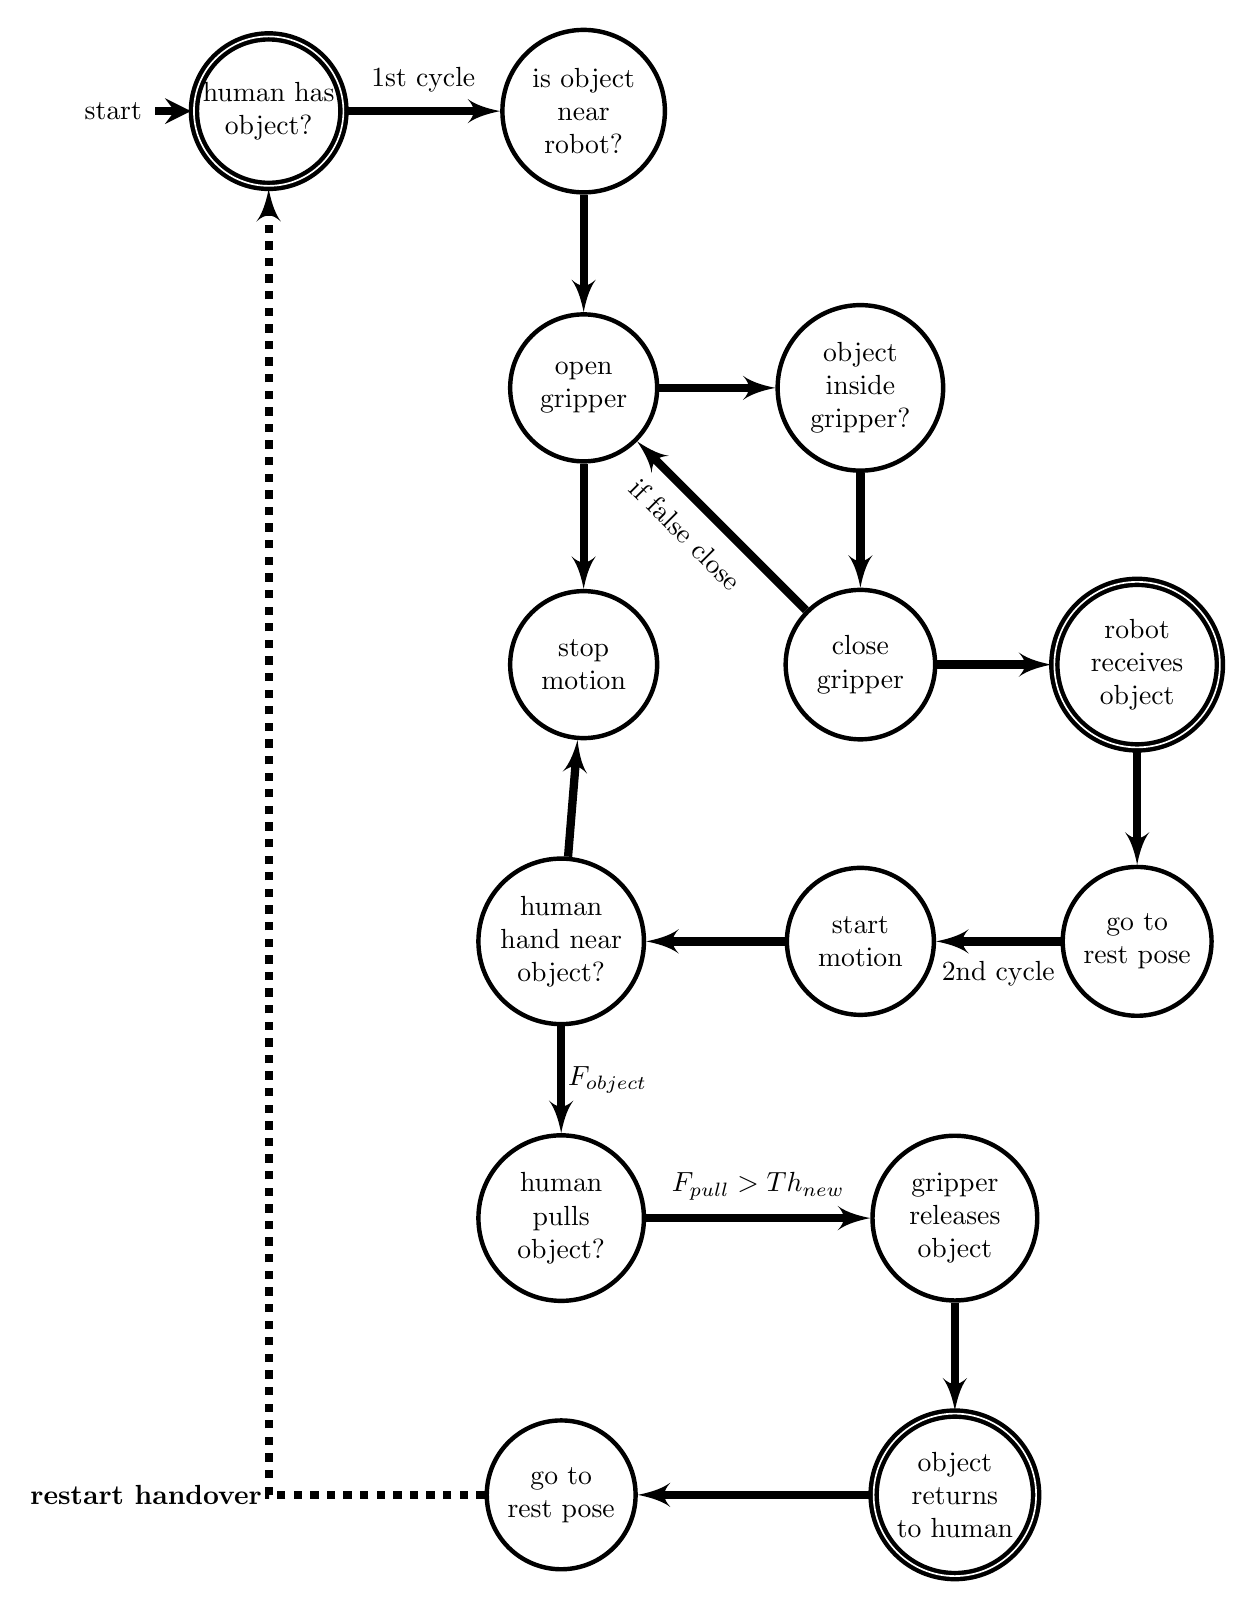
\begin{tikzpicture}[node distance=5cm, auto, scale = 1, ->,>=stealth, line width=3pt]
	
	\tikzstyle{cloud} = [draw,ultra thick, circle ,fill=white!20, text width=5em, text centered, node distance=10em, auto, inner sep=0pt, minimum height=2em]
	
	\tikzstyle{blank} = [circle ,fill=white!20, text width=5em, text centered, node distance=10em, auto, inner sep=0pt, minimum height=2em]
	
	\tikzstyle{line} = [draw, -latex', inner sep=1pt, minimum height=2em, node distance=10em]
	
	\node[cloud, initial, accepting] (human has object){human has object?};
	\node[cloud, node distance=4cm] (human hand is near?) [right of=human has object] {is object near robot?};
	\node[cloud] (open gripper) [below of=human hand is near?] {open gripper};
	\node[cloud] (stop motion) [below of=open gripper] {stop motion};
	\node[cloud] (object inside gripper?) [right of=open gripper] {object inside gripper?};
	\node[cloud] (close gripper) [below of=object inside gripper?] {close gripper};
	\node[cloud,accepting] (robot has object) [right of=close gripper] {robot receives object};		
	\node[cloud] (go rest pose) [below of=robot has object] {go to rest pose};
	\node[cloud] (start motion) [left of=go rest pose] {start motion};
	\node[cloud, node distance=3.8cm] (human hand is near again?) [left of=start motion] {human hand near object?};	
	\node[cloud] (pull handover object) [below of=human hand is near again?] {human pulls object?};
	\node[cloud, node distance=5cm] (open gripper release object) [right of=pull handover object] {gripper releases object};
	\node[cloud,accepting] (handover occurred) [below of=open gripper release object] {object returns to human};
	\node[cloud, node distance=5cm] (go rest pose2) [left of=handover occurred] {go to rest pose};
	
	\node[blank] (blank)[left of = go rest pose2]{};
	
	\path [line] (human has object) edge              node{1st cycle} (human hand is near?);
	\path [line] (human hand is near?) edge              node {} (open gripper);
	\path [line] (open gripper) edge              node {} (stop motion);
	\path [line] (open gripper) edge              node {} (object inside gripper?);
	\path [line] (object inside gripper?) edge   node {} (close gripper);
	\path [line] (close gripper) edge              node [near start, rotate=-45]{if false close} (open gripper);
	\path [line, node distance=6cm] (close gripper) edge node {}(robot has object);
	\path [line, node distance=6cm] (robot has object) edge node{} (go rest pose);
	
	\path [line] (go rest pose) edge              node {2nd cycle} (start motion);
	
	\path [line]  (start motion)edge               node {} (human hand is near again?);
	
	\path [line]  (human hand is near again?)edge               node {$F_{object}$}  (pull handover object);
	
	\path [line] (human hand is near again?) edge              node {} (stop motion);
	
	\path [line]  (pull handover object)edge               node {$F_{pull} >Th_{new}$} (open gripper release object);
	
	\path [line]  (open gripper release object)edge      node {}(handover occurred);
	\path [line]  (handover occurred)edge               node {}(go rest pose2);
	
	\path [line, dashed]  (go rest pose2) -|               node {\textbf{restart handover}}(human has object);
	
	
	\end{tikzpicture}
	\caption{Overview of human humanoid robot object handover Finite-State-Machine (FSM)}
\end{figure}


\clearpage
\section{both hands indiviudal- adding another hand}

the switching is based on the function which  uses hysteresis to compute relative position of object between human's hand and robot end-effectors 

\clearpage
\section{both hands together- using hands together}

\subsection{Variable object(s)}

\subsection{Constraint motion}

\subsection{Force Control changes}



\clearpage
\section{add a step-walk \& native stablizer}

\clearpage
\section{Repeat handover with step-walk}

\clearpage
\section{Experiments}

\clearpage
\section{Quantitative analysis}

\clearpage
\section{Results}

\clearpage
\section{Discussion}
%----an idea --have velocity proportional to the distance between robot ef and subj w.r.t. handover location

%the maths of rotation matrix look for relative rotation
%http://www.fastgraph.com/makegames/3drotation/

%page 11, 12  %http://web.cs.iastate.edu/~cs577/handouts/rotation.pdf

%wiki page ... {$https://en.wikipedia.org/wiki/Rotation_formalisms_in_three_dimensions$}

%3D to 2D rotation matrix reduction
%http://www.continuummechanics.org/rotationmatrix.html

%function ==direction-vector-to-rotation-matrix
%https://stackoverflow.com/questions/18558910/direction-vector-to-rotation-matrix

%vector direction link below
%${https://en.wikipedia.org/wiki/Direction_cosine}$

% ======================================================================= %
% ======================================================================= %

\chapter{Conclusion Discussion/Future possibilities}


\section{A Section}


\subsection{A Subsection}


\section{Another Section}



% ======================================================================= %
% ======================================================================= %







%% ----------------------------------------------------------------
% Now begin the Appendices, including them as separate files

\addtocontents{toc}{\vspace{2em}} % Add a gap in the Contents, for aesthetics

\appendix % Cue to tell LaTeX that the following 'chapters' are Appendices

\input{Appendices/Appendix-morethan}\label{morethan}

\chapter{Appendix: distinct motor contagion}
\label{distinct}

\chapter{Appendix: Handover}

\begin{lstlisting}[language=C++,basicstyle=\footnotesize, caption={wrench}]
const sva::ForceVecd 
ForceSensor::wrenchWithoutGravity(const mc_rbdyn::Robot & robot) const
{
sva::PTransformd X_0_p = 
robot.mbc().bodyPosW[robot.bodyIndexByName(parentBody_)];
auto w = wrench_ - calibration_->wfToSensor(X_0_p, X_p_f_);
return w;
}

sva::ForceVecd 
ForceSensor::worldWrench(const mc_rbdyn::Robot & robot) const
{
sva::ForceVecd w_fsactual = wrench();
sva::PTransformd X_parent_0 = 
robot.mbc().bodyPosW[robot.bodyIndexByName(parentBody_)].inv();
sva::PTransformd X_fsactual_0 = X_parent_0 * X_fsactual_parent();
return X_fsactual_0.dualMul(w_fsactual);
}

sva::ForceVecd 
ForceSensor::worldWrenchWithoutGravity(const mc_rbdyn::Robot & robot) const
{
sva::ForceVecd w_fsactual = wrenchWithoutGravity(robot);
sva::PTransformd X_parent_0 = 
robot.mbc().bodyPosW[robot.bodyIndexByName(parentBody_)].inv();
sva::PTransformd X_fsactual_0 = X_parent_0 * X_fsactual_parent();
return X_fsactual_0.dualMul(w_fsactual);
}
\end{lstlisting}\label{handover}

\addtocontents{toc}{\vspace{2em}}  % Add a gap in the Contents, for aesthetics

\backmatter

%% ----------------------------------------------------------------
\label{Bibliography}
\lhead{\emph{Bibliography}}  % Change the left side page header to "Bibliography"
\bibliographystyle{unsrtnat}  % Use the "unsrtnat" BibTeX style for formatting the Bibliography
\bibliography{bib}  % The references (bibliography) information are stored in the file named "bib.bib"



\end{document}  % The End
%% ----------------------------------------------------------------